\documentclass[conference,compsoc]{IEEEtran}
\usepackage[utf8]{inputenc}
\usepackage{amsmath,amssymb}
\usepackage[ruled,vlined]{algorithm2e}
\usepackage{enumitem}
\usepackage{hyperref}
\usepackage{graphicx}
\usepackage{booktabs}
\usepackage{listings}
\usepackage{multirow}
\usepackage{textcomp}
\usepackage{xcolor}
\usepackage{kotex}
\usepackage{tikz}
\usepackage{pgfplots}
\usepackage{tcolorbox}

\usetikzlibrary{shapes,arrows,positioning,fit,calc}
\providecommand{\tightlist}{\setlength{\itemsep}{0pt}\setlength{\parskip}{0pt}}

\begin{document}
\title{PatchScribe: Theory-Guided Vulnerability Repair with Dual Causal Explanations}

\author{\IEEEauthorblockN{Anonymous Authors}}
\maketitle
\begin{abstract}
Software vulnerabilities require rapid patching, yet current LLM-based repair achieves only 22--26\% correctness due to lack of causal grounding. We present PatchScribe, a theory-guided framework that combines pre-hoc causal formalization with post-patch consistency validation. We focus on memory-safety vulnerabilities (buffer overflows, use-after-free, null-pointer dereferences), which constitute 92\% of our evaluation dataset and represent a critical class of exploitable bugs in C programs. PatchScribe constructs Program Causal Graphs and Structural Causal Models to systematically identify vulnerability conditions, then guides LLM synthesis with explicit intervention catalogs. Dual explanations ($E_{\text{bug}}$, $E_{\text{patch}}$) enable machine-assisted validation of causal consistency. Evaluation on 121 real-world CVEs shows PatchScribe improves correctness from 39.7\% (structured baseline) to 67.8\% (+28.1 percentage points), or +41.4pp over raw LLM approaches (26.4\%), with 91.9\% precision and practical deployment latency (73.93s average). Our approach offers semi-formal assurance of causal path disruption for memory-safety vulnerabilities, demonstrating that systematic causal reasoning can enhance trustworthiness of semi-automated security tooling with human-in-the-loop pattern refinement.
\end{abstract}
\section{Introduction}\label{introduction}

Software vulnerabilities in critical infrastructure can lead to data breaches and system compromises~\cite{verizon2024dbir}. The average time from vulnerability disclosure to patch deployment spans weeks~\cite{wang2025vulnrepaireval}, creating exposure windows that adversaries may exploit. As codebases grow and attack surfaces expand, security teams need to accelerate patch development without sacrificing correctness~\cite{neuhaus2007predicting}.

Large language models (LLMs) can potentially automate patch generation~\cite{wang2025vulnrepaireval,nong2025appatch}. Given a vulnerability description and surrounding code context, recent models can draft candidate patches within minutes~\cite{nong2024automatedvulnpatch}. This capability has generated research activity in LLM-based automated program repair, with recent benchmarks evaluating models across hundreds of real-world CVEs~\cite{wang2024sok}.

This work focuses on memory-safety vulnerabilities in C---a critical domain where memory-safety bugs constitute approximately 40\% of CVE entries~\cite{nsa2022softwaresafetymemory}, including buffer overflows (CWE-119, CWE-787), use-after-free (CWE-416), and null-pointer dereferences (CWE-476). We concentrate on this vulnerability class because it exhibits deterministic causal relationships amenable to formal modeling through program dependence analysis and symbolic reasoning. Our evaluation dataset reflects this focus (92\% memory-safety bugs), enabling rigorous validation of the causal formalization framework. Extension to logic flaws, concurrency bugs, and type confusion vulnerabilities is discussed in \S\ref{sec:discussion}.

However, current evaluations show limitations: exploit-grounded assessment of GPT-4 on 156 real CVEs across Linux, Chromium, and other OSS projects shows only 22\% of generated patches eliminate the vulnerability without collateral damage~\cite{wang2025vulnrepaireval}. Our baseline evaluation on 121 CVEs confirms similar limitations, with raw LLM approaches achieving only 26.4\% patch correctness. These findings indicate that the accuracy gap is systemic rather than dataset-specific.

One factor contributing to this limitation is the absence of \emph{causal grounding}~\cite{ullah2024secLLMHolmes}.
Current post-hoc approaches validate patches empirically (pass tests, block exploits) but provide no systematic evidence that all causal paths to exploitation are disrupted. Traditional LLM-based repair follows this paradigm: generate a plausible patch, then validate whether it passes tests or blocks known exploits~\cite{kulsum2024case}. Without formal causal models, patch acceptance relies on trust rather than verification. Security reviewers must independently verify the vulnerability's root cause and assess whether the changes address all attack vectors, reducing automation benefits.

We address this limitation through \emph{pre-hoc causal formalization}---an alternative approach where vulnerability causality is explicitly modeled \emph{before} patch synthesis. PatchScribe implements a hybrid approach combining pre-hoc formalization with post-patch consistency validation through three mechanisms. First, it constructs a Program Causal Graph (PCG) that captures the predicates enabling exploitation, including missing security checks, unsafe data flows, and vulnerable control paths. Second, it instantiates a Structural Causal Model (SCM) that formalizes these predicates as structural equations and enumerates interventions capable of disrupting them. Third, it packages this formal analysis into a structured bug explanation ($E_{\text{bug}}$) that guides LLM-based synthesis while constraining the solution space to causally sound interventions.

\begin{figure*}[t]
\centering
\resizebox{0.95\textwidth}{!}{
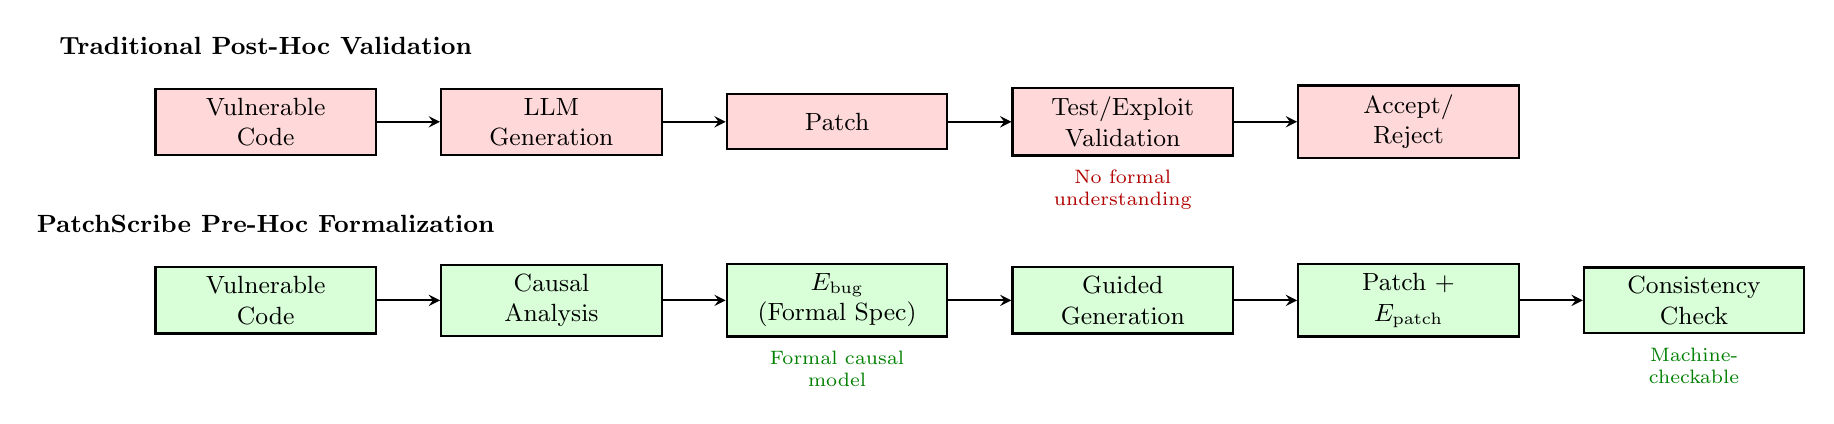
\begin{tikzpicture}[
  node distance=0.4cm and 0.8cm,
  box/.style={rectangle, draw, thick, minimum width=2.8cm, minimum height=0.7cm, font=\small, align=center},
  posthoc/.style={box, fill=red!15},
  prehoc/.style={box, fill=green!15},
  arrow/.style={->, >=stealth, thick},
  label/.style={font=\small\bfseries}
]

% Post-hoc approach (top)
\node[label] (post-label) at (0, 0) {Traditional Post-Hoc Validation};
\node[posthoc, below=0.3cm of post-label] (post1) {Vulnerable\\Code};
\node[posthoc, right=of post1] (post2) {LLM\\Generation};
\node[posthoc, right=of post2] (post3) {Patch};
\node[posthoc, right=of post3] (post4) {Test/Exploit\\Validation};
\node[posthoc, right=of post4] (post5) {Accept/\\Reject};

\draw[arrow] (post1) -- (post2);
\draw[arrow] (post2) -- (post3);
\draw[arrow] (post3) -- (post4);
\draw[arrow] (post4) -- (post5);

\node[below=0.05cm of post4, font=\scriptsize, text=red!70!black, text width=2.5cm, align=center] {No formal\\understanding};

% Pre-hoc approach (bottom)
\node[label, below=1.8cm of post-label] (pre-label) {PatchScribe Pre-Hoc Formalization};
\node[prehoc, below=0.3cm of pre-label] (pre1) {Vulnerable\\Code};
\node[prehoc, right=of pre1] (pre2) {Causal\\Analysis};
\node[prehoc, right=of pre2] (pre3) {$E_{\text{bug}}$\\(Formal Spec)};
\node[prehoc, right=of pre3] (pre4) {Guided\\Generation};
\node[prehoc, right=of pre4] (pre5) {Patch +\\$E_{\text{patch}}$};
\node[prehoc, right=of pre5] (pre6) {Consistency\\Check};

\draw[arrow] (pre1) -- (pre2);
\draw[arrow] (pre2) -- (pre3);
\draw[arrow] (pre3) -- (pre4);
\draw[arrow] (pre4) -- (pre5);
\draw[arrow] (pre5) -- (pre6);

\node[below=0.05cm of pre3, font=\scriptsize, text=green!50!black, text width=2.5cm, align=center] {Formal causal\\model};
\node[below=0.05cm of pre6, font=\scriptsize, text=green!50!black, text width=2.5cm, align=center] {Machine-\\checkable};

\end{tikzpicture}
}
\caption{Comparison of traditional post-hoc validation and PatchScribe's pre-hoc formalization approach. Traditional approaches (left) validate patches post-hoc via testing, providing no formal understanding of causal paths. PatchScribe (right) constructs formal causal specifications pre-hoc to guide LLM synthesis, then validates via machine-checkable dual-explanation consistency checking.}
\label{fig:pre-post-hoc}
\end{figure*}

After the model proposes a patch, PatchScribe performs machine-assisted consistency validation by extracting a complementary patch explanation ($E_{\text{patch}}$) and comparing it against the original causal model. This dual-explanation framework enables systematic verification along three dimensions: \emph{coverage} (whether the patch addresses all identified causal paths), \emph{intervention presence} (whether prescribed actions were implemented), and \emph{completeness} (whether additional undocumented changes exist). A calibrated checker synthesizes these dimensions into one of three verdicts---PASS, REVIEW, or FAIL---with thresholds tuned to balance precision and recall. In our evaluation, approximately 65\% of patches receive PASS verdicts, while those requiring manual review or triggering alternative strategies maintain consistent evaluation criteria through cached causal artifacts.

This approach supports practical deployment integration. The framework operates in two phases: Phase~1 performs one-time formalization per CVE (PCG/SCM construction averaging 0.30 seconds), caching artifacts for reuse. Phase~2 validates each candidate patch through guided generation (averaging 6.83 seconds) and consistency checking, with total system time averaging 73.93 seconds (median 75.72 seconds). The system achieves high throughput with 1.48 average iterations per case and maintains practical resource usage with peak memory averaging 12.5 MB. All verdicts reference the same cached causal artifacts, enabling consistent evaluation criteria.


This paper makes three contributions:
\begin{enumerate}[leftmargin=*]
  \item \textbf{Conceptual---pre-hoc causal formalization.} We show how PCGs and SCMs guide patch synthesis before code generation, improving correctness from 26.4\% (raw LLM baseline) to 67.8\% across 121 CVEs---a +41.4 percentage point gain representing 157\% relative improvement while holding exploit-replay evaluation constant.
  \item \textbf{Technical---consistency checking.} We design dual explanations ($E_{\text{bug}}$, $E_{\text{patch}}$) and a three-dimensional checker (coverage, intervention, completeness) that maintains practical deployment latency with mean runtime of 73.93 seconds.
  \item \textbf{Empirical---expert validation.} Manual evaluation by four professional security engineers demonstrates that PatchScribe's explanations improve patch assessment quality across all dimensions (accuracy: 4.3/5.0, completeness: 4.1/5.0, causality: 4.3/5.0) and provide clear causal rationale for deployment decisions.
\end{enumerate}

Section~\ref{sec:background} motivates the pre-hoc approach and summarizes our design requirements; Sections~\ref{sec:approach}--\ref{sec:system} describe the framework and system; Section~\ref{sec:evaluation} reports empirical results; Sections~\ref{sec:related}--\ref{sec:conclusion} conclude with related work and limitations.

\begin{table}[t]
\centering
\caption{Design requirements for theory-guided patch generation.}
\label{tab:requirements}
\small
\begin{tabular}{@{}p{0.12\columnwidth}p{0.82\columnwidth}@{}}
\toprule
\multicolumn{2}{@{}l}{\textbf{Core Causal Assurance}} \\
\midrule
R1 & \textbf{Formalization Quality:} Precisely characterize vulnerability conditions and their causal dependencies through formal models. \\
R2 & \textbf{Causal Consistency:} Validate that patch interventions logically eliminate vulnerability conditions across all identified causal paths. \\
R3 & \textbf{Dual Explanation:} Generate structured explanations for both the vulnerability ($E_{\text{bug}}$) and the patch ($E_{\text{patch}}$), enabling systematic comparison. \\
R4 & \textbf{Consistency Validation:} Provide machine-assisted consistency checking between $E_{\text{bug}}$ and $E_{\text{patch}}$ through calibrated metrics (Jaccard $\geq$ 0.3, location accuracy $<$ 5\%); accept conservative rejections over unvalidated claims. \\
\midrule
\multicolumn{2}{@{}l}{\textbf{Practical Usability}} \\
\midrule
R5 & \textbf{Coverage:} Capture vulnerability-relevant conditions via data-flow, control-flow, and security pattern analyses. \\
R6 & \textbf{Usability:} Present formal specifications alongside natural-language summaries mapped to concrete code locations. \\
R7 & \textbf{Workflow Compatibility:} Integrate with standard toolchains (Clang/LLVM) and maintain practical runtimes. \\
R8 & \textbf{Regression:} Execute test suites to detect patches that inadvertently break existing functionality. \\
\bottomrule
\end{tabular}
\end{table}

\section{Background and Motivation}\label{sec:background}

\subsection{LLM-Based Vulnerability Repair}

LLM-based repair pipelines can potentially provide rapid response, yet exploit-grounded benchmarks show that recent models fix only 22\% of CVEs~\cite{wang2025vulnrepaireval}. Our evaluation confirms this challenge, with baseline LLM approaches achieving 26.4\% correctness on 121 CVEs. Current approaches lack formal evidence: natural-language rationales and limited tests do not demonstrate whether all causal paths to the bug have been disrupted, so reviewers must verify the root cause and check whether variant exploits remain~\cite{ullah2024secLLMHolmes}.

\noindent\textbf{Why pre-hoc?} Patch acceptance decisions require causal reasoning---reviewers need to know which predicates enabled the vulnerability and whether the patch disrupts them~\cite{Wu2023mitigating, xiong2018identifying}. PatchScribe constructs a Program Causal Graph (PCG) and Structural Causal Model (SCM) before invoking the LLM, injects that structured context into the prompt, and validates that the resulting intervention aligns with the same formal objects.


\begin{figure*}[t]
  \centering
  \includegraphics[width=0.95\textwidth]{figures/overview.png}
  \caption{PatchScribe's dual-phase pipeline. Phase~1 formalizes the vulnerability once per CVE; Phase~2 uses that formal specification for guided synthesis and machine-assisted acceptance.}
  \label{fig:overview}
\end{figure*}

\noindent\textbf{Operational risk.} Deploying unverifiable patches may create unwarranted confidence~\cite{fei2025patchcorrectness}. By mapping every edit to explicit causal paths, PatchScribe produces machine-checkable artifacts that reviewers can audit and reuse when the same CVE reappears. Figure~\ref{fig:pre-post-hoc} contrasts the ``generate-then-test'' loop with our pre-hoc workflow that caches formal analyses, guides synthesis, and enforces consistency before acceptance.

\subsection{Design Requirements}

Table~\ref{tab:requirements} summarizes the constraints that guided PatchScribe's design. R1--R4 ensure causal assurance (precise formalization, dual explanations, calibrated acceptance), while R5--R8 keep the workflow practical for LLVM-based pipelines and developer-facing artifacts.

\section{Approach Overview}\label{sec:approach}

PatchScribe runs in two tightly coupled phases (Figure~\ref{fig:overview}). Phase~1 formalizes the vulnerability once per CVE; Phase~2 consumes that formal specification for guided synthesis and validation. Keeping the same causal objects throughout the workflow ensures that generation and checking reason about identical predicates.

\noindent\textbf{Phase 1: Formalization.}
\begin{enumerate}[leftmargin=*,nosep]
  \item \textit{Backward slicing:} extract vulnerability-relevant statements using Clang/LLVM and sanitizer metadata~\cite{chalupa2020dg}.
  \item \textit{PCG construction:} fuse data-flow, control-flow, and pattern detectors to build causal nodes/edges; transitive reduction keeps graphs compact~\cite{aho1972thetransitive}.
  \item \textit{SCM instantiation:} map PCG nodes to structural equations and intervention options, producing counterfactual predicates~\cite{neuberg2003causality}.
  \item \textit{$E_{\text{bug}}$ package:} emit a structured artifact containing logical conditions, natural-language summaries, code links, and suggested interventions that will seed the LLM prompt.
\end{enumerate}

\noindent\textbf{Phase 2: Guided synthesis + checking.}
\begin{enumerate}[leftmargin=*,nosep]
  \item Embed $E_{\text{bug}}$ into the prompt alongside the vulnerable snippet, plus reminders about the acceptance policy (PASS/REVIEW/FAIL).
  \item Interpret the LLM diff as interventions, generating $E_{\text{patch}}$ that describes which causal paths were disrupted.
  \item Run the three-dimensional consistency checker (coverage, intervention presence, completeness) with calibrated thresholds (0.85 accept, 0.70--0.85 review, $<0.70$ reject).
  \item Either accept the patch with machine-checkable evidence, provide structured feedback for another attempt, or fall back to manual review. Iterative refinement is capped at five attempts (§\ref{sec:system}).
\end{enumerate}

PatchScribe reasons about vulnerabilities using two compact mathematical objects: the Program Causal Graph (PCG) and the Structural Causal Model (SCM)~\cite{neuberg2003causality}. Table~\ref{tab:notation} (Appendix~\ref{app:notation}) summarizes notation, and Algorithm~\ref{alg:pcg}/Algorithm~\ref{alg:consistency} in Appendix~\ref{app:algorithms} detail construction and checking procedures.

\subsection{Program Causal Graphs}\label{program-causal-graph-pcg}

A PCG is a directed graph $G = (V, E)$ that captures how predicates and events inside the slice influence the vulnerability node $V_{\text{bug}}$. Nodes represent conditions (e.g., ``input len $> 256$''), security checks (presence/absence), or events (function calls, memory writes); edges encode direct causal influence derived from control- and data-dependence plus security-pattern detectors. Typical graphs contain 10--25 nodes and 15--40 edges after transitive reduction, keeping reasoning tractable.

\textbf{Illustrative Example.} Consider a simplified buffer overflow vulnerability:
\begin{lstlisting}[language=C, basicstyle=\ttfamily\small, numbers=none]
void process(char *input, int len) {
  char buf[256];
  memcpy(buf, input, len);  // vulnerable line
}
\end{lstlisting}
PCG construction identifies four key nodes: (1) $v_1$: ``\texttt{len > 256}'' (attacker-controlled predicate from backward slicing on \texttt{len}), (2) $v_2$: ``\texttt{!bound\_check(len, 256)}'' (absent security check detected via pattern matching against our 32-template library), (3) $v_3$: ``\texttt{memcpy} with unbounded \texttt{len}'' (vulnerable operation from data-flow analysis), (4) $v_{\text{bug}}$: ``buffer overflow'' (vulnerability node). Edges capture causal dependencies: $v_1 \to v_3$ (data-flow: \texttt{len} influences copy size), $v_2 \to v_3$ (control-flow: missing check enables unsafe operation), $v_3 \to v_{\text{bug}}$ (direct causation). The SCM structural equation formalizes: $C_{\text{overflow}} := (C_{\text{len>256}} \land \neg C_{\text{bound\_check}} \land C_{\text{memcpy\_unbounded}})$. Suggested interventions include $\text{do}(C_{\text{bound\_check}} = \text{true})$ (add \texttt{if (len > 256) return;}) or $\text{do}(C_{\text{len}} = \min(\text{len}, 256))$ (sanitize input before copy). This formalization guides LLM generation while constraining solutions to causally sound edits.

Algorithmic details for multi-analyzer fusion and absence-node detection appear in Algorithm~\ref{alg:pcg} (Appendix); the complete pattern library for detecting missing security checks is provided in Appendix~\ref{app:patterns}.

\subsection{Structural Causal Model}

The SCM maps each PCG node $v$ to a variable $C_v$ with a structural equation $C_v := f_v(\text{Parents}(v))$. Exogenous variables $\mathcal{X}$ capture attacker-controlled inputs; endogenous variables $\mathcal{C}$ encode program predicates; interventions are Pearl-style $\text{do}(X=x)$ operations that sever incoming edges. The vulnerability predicate is expressed as $V_{\text{bug}} := \bigwedge_{C_j \in \mathcal{P}} C_j$, enabling counterfactual reasoning over interventions. Appendix~\ref{app:scm-templates} provides detailed SCM templates for common vulnerability classes with structural equations and intervention options.

\subsection{Dual Explanations}

\textbf{$E_{\text{bug}}$} bundles (i) the logical condition for $V_{\text{bug}}$, (ii) annotated code spans for each predicate, (iii) causal paths $\Pi_{\text{bug}}$, and (iv) an intervention catalogue $\mathcal{I}_{\text{bug}}$ that enumerates safe edits (add guard, sanitize input, reorder control).
\textbf{$E_{\text{patch}}$} interprets the diff returned by the LLM as interventions, records which causal paths are disrupted, and maps edits back to code locations. These dual artifacts keep human reviewers and the checker aligned on the same semantics.

\subsection{Consistency Objectives}

The checker compares $E_{\text{bug}}$ and $E_{\text{patch}}$ along three dimensions.

\textbf{Coverage ($s_c$).} every path $\pi \in \Pi_{\text{bug}}$ identified through pattern-based analysis must contain a disrupted node or edge. While our 32 security patterns achieve 90\% F1 score, coverage is necessarily bounded by pattern library completeness. Appendix~\ref{app:pcg-metrics} reports 96.2\% node recall across evaluated CVEs, demonstrating comprehensive capture of vulnerability-relevant program structure.

\textbf{Intervention Presence ($s_i$).} the diff must realize one of the prescribed interventions for each violated predicate.

\textbf{Completeness ($s_{\text{comp}}$).} the patch must not introduce new vulnerability patterns (checked via negative templates).

Scores are combined as $s_{\text{total}} = 0.5s_c + 0.35s_i + 0.15s_{\text{comp}}$; thresholds at $0.85$ (accept), $0.70$--$0.85$ (manual review), and $<0.70$ (reject) yield 91.9\% precision and 91.4\% recall on 121 CVEs (§\ref{sec:evaluation}). Logistic-regression calibration, ROC curves, and ablation analyses are deferred to Appendix~\ref{app:threshold-details}.
\section{PatchScribe System}\label{sec:system}

The implementation treats PCG/SCM artifacts as first-class build products: Phase~1 runs once per CVE and is cached, while Phase~2 reuses those artifacts for every LLM attempt.

\subsection{Phase 1: Building $E_{\text{bug}}$}

\noindent\textbf{Predicate extraction.} Each slice statement becomes a predicate node annotated with file/line metadata, enabling precise hyperlinks inside the artifact.

\noindent\textbf{Causal structuring.} The PCG builder merges data-flow, control-flow, and absence-pattern detectors to form $\Pi_{\text{bug}}$; statistics (node/edge counts, refinement history) are logged for auditing.

\noindent\textbf{SCM instantiation.} Structural equations are emitted in both human-readable math and SMT-friendly JSON so that downstream tools can perform optional solver checks when time allows. Appendix~\ref{app:scm-templates} details the templates used for instantiation across different vulnerability classes.

\noindent\textbf{Artifact packaging.} $E_{\text{bug}}$ includes the logical formula for $V_{\text{bug}}$, per-node natural-language glosses, example traces, and a prescriptive intervention catalog $\mathcal{I}_{\text{bug}}$ (``insert bounds check before line 42'').

All components are cacheable; evaluating three models against the same CVE reuses the identical $E_{\text{bug}}$ without recomputing analyses.

\subsection{Phase 2: Guided generation and acceptance}

\noindent\textbf{Prompting.} The LLM receives the vulnerable slice, $E_{\text{bug}}$, and a reminder that only patches passing the consistency checker are accepted. Detailed prompt structures for all experimental conditions are provided in Appendix~\ref{app:prompts}.

\noindent\textbf{Diff interpretation.} A lightweight analyzer converts the diff into interventions (guards, sanitization, error propagation) and produces $E_{\text{patch}}$ by marking disrupted paths.

\noindent\textbf{Consistency scoring.} Algorithm~\ref{alg:consistency} (Appendix~\ref{app:algorithms}) computes the four sub-scores and aggregates them into $s_{\text{total}}$.

\noindent\textbf{Outcome handling.} Patches with $s_{\text{total}} \geq 0.85$ are auto-accepted and logged with their dual explanations; scores in $[0.70, 0.85)$ trigger reviewer notifications with pinpointed missing evidence; lower scores prompt automatic re-prompting (up to five attempts) before handing control to a human.

The workflow mirrors real deployment practice: dual explanations and the PASS/REVIEW/FAIL verdict are published in CI dashboards, while Appendix~\ref{app:rubric} supplies the rubric used by human evaluators when manual review is requested.
\section{Evaluation}\label{sec:evaluation}

We evaluate PatchScribe along multiple dimensions to answer the following key research questions:

\noindent\textbf{RQ1: Theory-Guided Generation Effectiveness.} Does pre-hoc formal bug specification \(E_{\text{bug}}\) lead to more accurate patches than post-hoc explanations or vague hints? How much does theory-guided prompting with precise formal specifications improve patch quality compared to traditional approaches?

\noindent\textbf{RQ2: Patch Quality.} What is the quality of patches generated by the theory-guided approach? We assess patches along three dimensions: (1) \emph{correctness}---whether the patch eliminates the vulnerability without introducing regressions, verified through manual security review by four expert evaluators; (2) \emph{ground truth similarity}---AST-based structural comparison with developer-authored CVE fixes to measure alignment with real-world solutions; and (3) \emph{vulnerability elimination rate}---percentage of patches that successfully block all known exploit paths, validated via PoC execution when available. These metrics collectively evaluate whether PatchScribe produces deployable, high-fidelity patches.

\begin{table}[t]
  \centering
  \caption{Dataset statistics by vulnerability type, programming language, and code complexity.}
  \label{tab:dataset-stats}
  \small
  \resizebox{0.48\textwidth}{!}{

    \begin{tabular}{lcc}
    \toprule
    \textbf{Characteristic} & \textbf{Zeroday Repair} & \textbf{ExtractFix} \\
    \midrule
    \textbf{Total CVEs} & 97 & 24 \\
    \textbf{Programming Language} & C & C \\
    \midrule
    \multicolumn{3}{l}{\textit{Vulnerability Types (CWE)}} \\
    \quad CWE-125 (OOB Read) & 23 (25\%) & 9 (38\%) \\
    \quad CWE-190 (Int Overflow) & 11 (11\%) & 6 (25\%) \\
    \quad CWE-476 (NULL Deref) & 25 (26\%) & 2 (8\%) \\
    \quad CWE-787 (OOB Write) & 17 (17\%) & 7 (29\%) \\
    \quad CWE-401 (Missing release) & 11 (11\%) & - \\
    \quad CWE-457 (Uninitialized var.) & 10 (10\%) & - \\
    \midrule
    \multicolumn{3}{l}{\textit{Code Complexity (Lines of Code)}} \\
    \quad Total Files & 97 & 24 \\
    \quad Total LOC & 6,088 & 2,466 \\
    \quad Simple ($\leq$50 LoC) & 49 (51\%) & 8 (33\%) \\
    \quad Medium (50--100 LoC) & 35 (36\%) & 9 (38\%) \\
    \quad Complex ($\geq$100 LoC) & 13 (13\%) & 7 (29\%) \\
    \quad Range & [7, 517] & [20, 452] \\
    \quad Mean $\pm$ Std & $62.76 \pm 63.65$ & $102.75 \pm 98.55$ \\
    \bottomrule
    \end{tabular}
  }
\end{table}

\noindent\textbf{RQ3: Scalability and Performance.} What is the time overhead of the two-phase workflow, and is it acceptable for practical deployment? We measure: (1) \emph{phase-wise breakdown}---separate timing for Phase~1 (PCG/SCM construction) and Phase~2 (guided generation + consistency checking) to identify bottlenecks; (2) \emph{total system time}---end-to-end latency per CVE; (3) \emph{iteration count}---average number of patch generation attempts before acceptance, indicating guidance effectiveness; and (4) \emph{resource usage}---peak memory consumption and analysis overhead to assess hardware requirements. Results are stratified by code complexity (simple: $<$50 LoC, medium: 50--100 LoC, complex: $>$100 LoC) to evaluate scalability across different vulnerability sizes.

\noindent\textbf{RQ4: Explanation Quality.} How well do dual causal explanations support human reviewers in understanding vulnerabilities and assessing patches? We evaluate explanation quality through: (1) \emph{checklist-based coverage}---automated detection of required elements (vulnerability type, root cause, formal condition, intervention description) to ensure completeness; and (2) \emph{expert quality scores}---four security professionals rate $E_{\text{bug}}$ and $E_{\text{patch}}$ on a 1--5 Likert scale across four dimensions (accuracy, completeness, clarity, causality) using a structured rubric (Appendix~\ref{app:rubric}). Comparing PatchScribe's causal explanations against baseline post-hoc narratives (C1) reveals whether formal SCM-based reasoning improves reviewer understanding and deployment confidence. The same four experts performed all manual assessments (RQ1, RQ2, RQ4) to ensure consistency.

\subsection{Experimental Setup}

\subsubsection{Datasets}

We evaluate PatchScribe on two complementary vulnerability repair benchmarks covering memory safety and diverse vulnerability types. Table~\ref{tab:dataset-stats} summarizes dataset characteristics.

\noindent\textbf{Zero-Day.} We use the Zero-Day dataset from the APPATCH study~\cite{nong2025appatch}, comprising 97 recent (2024) CVEs concentrated on memory-safety bugs in C codebases; exploit metadata exists for 64\% of cases. It stresses depth by keeping the vulnerability family constant.

\noindent\textbf{ExtractFix.} We adopt the ExtractFix dataset from the APPATCH study~\cite{nong2025appatch}, consisting of 24 curated CVEs spanning six CWE families in C with paired PoCs and ground-truth patches; it stresses breadth across diverse vulnerability types.

We therefore evaluate across 121 CVEs covering both homogeneous depth and heterogeneous breadth.

\subsubsection{Baselines and Ablations}

We compare PatchScribe across four configurations: C1 (baseline raw LLM with no formal guidance), C2 (vague hints delivered as informal prompts), C3 (pre-hoc guidance using \(E_{\text{bug}}\) without consistency checking), and C4 (the full PatchScribe pipeline with consistency checking). Appendix~\ref{app:prompts} provides the complete prompt templates for each configuration.
We compare against APPATCH~\cite{nong2025appatch} using their published results on the same datasets.

We acknowledge that C1 represents a minimalist baseline. However, this design choice reflects real-world deployment scenarios where developers often lack structured CVE analysis: our baseline mirrors the information available to rapid-response teams without security-focused tooling. Prior work (APPATCH) similarly evaluates raw LLM performance as a baseline. Moreover, our comparison with APPATCH (Table~\ref{tab:comparison}), which uses curated prompts, provides an additional reference point beyond the C1 baseline, demonstrating PatchScribe's effectiveness against state-of-the-art approaches.

\subsubsection{Evaluation Metrics}

For RQ1 (Theory-Guided Generation):
(1) Patch correctness rate -- patches successfully addressing vulnerabilities through manual evaluation;
(2) Ground truth similarity -- comparing generated patches to actual CVE fixes using AST-based structural similarity;
(3) First-attempt success rate -- measuring how often the initial LLM response is correct, indicating guidance quality.
We conduct an ablation study with four conditions:
C1 (no guidance: raw LLM with no formal specification), C2 (vague hints: informal prompts like ``add a check''), C3 (abstract guidance: general vulnerability description), and C4 (full PatchScribe with \(E_{\text{bug}}\) formal specification).
Comparing C1 vs C4 shows the overall impact of theory-guided generation, while intermediate conditions isolate specific contributions. Complete prompt templates and design rationale are detailed in Appendix~\ref{app:prompts}.

For RQ2 (Patch Quality), we measure:
(1) Patch correctness through manual evaluation using structured assessment;
(2) Ground truth similarity -- comparing generated patches to actual CVE fixes using AST-based structural similarity;
(3) Vulnerability elimination rate -- patches that successfully remove the identified vulnerabilities.
We assess patch quality through structured manual evaluation, focusing on whether patches correctly address vulnerabilities and how closely they align with ground truth fixes.

For RQ3 (Scalability and Performance), we measure:
(1) Time breakdown by phase -- separately measuring formalization (Phase 1) and generation (Phase 2) time;
(2) Total system time per vulnerability;
(3) Iteration count -- average number of patch generation attempts before success;
(4) Resource usage -- peak memory and analysis overhead.
We stratify results by code complexity (simple: \(\textless\) 50 LoC, medium: 50-100 LoC, complex: \(\textgreater\) 100 LoC) to assess scalability.

For RQ4 (Explanation Quality), we measure:
(1) Checklist-based coverage -- automated detection of required elements (vulnerability type, root cause, formal condition, intervention description);
(2) Expert quality scores -- four security professionals rate \(E_{\text{bug}}\) and \(E_{\text{patch}}\) on accuracy, completeness, clarity, and causality (1-5 Likert scale) using a structured rubric.
The same four experts also performed manual correctness evaluation for RQ1 and RQ2, ensuring consistency across all manual assessments.

\subsubsection{Implementation Details and Reproducibility}

\textbf{Computing Environment.}
All experiments executed on Ubuntu 22.04 servers (Intel Xeon Silver 4510, 4.1GHz, 48 cores, 448GB RAM). No GPU required. (121 CVEs $\times$ 4 conditions $\times$ 3 independent runs).

\noindent\textbf{LLM Configuration.}
We used three LLM providers: OpenAI API v1 (GPT-5-mini)~\cite{openai}, Anthropic API (Claude Haiku 4.5)~\cite{anthropic}, and Google Gemini API (Gemini 2.5 Flash)~\cite{gemini}. The context window was set to 8192 tokens (output maximum). Each LLM request had a timeout of 180 seconds with exponential backoff retry (maximum 3 attempts). To handle concurrent requests efficiently, we configured 50 parallel requests via a connection pool (50 connections, 500 maximum).

\noindent\textbf{Analysis Pipeline Configuration.}
For backward slicing, we employed Clang/LLVM 14.0~\cite{lattner2004llvm} with BFS traversal and unlimited depth, resulting in an average of 45 statements per slice. PCG construction utilized 32 security check patterns (CWE-based) with transitive reduction enabled, producing an average of 18.7 nodes per graph. SCM reasoning was performed using Z3 4.12.0 for intervention planning, with symbolic execution disabled in production to prevent solver timeouts~\cite{de2008z3}. We applied consistency thresholds requiring Jaccard similarity $\geq$ 0.3, location accuracy $<$ 5 \%, and causal coverage $\geq$ 67\% (4/6 checks passing).

\noindent\textbf{Evaluation Protocol.}
We conducted three independent runs using random seeds 42, 123, and 7220, with results averaged and standard deviation reported. Manual assessment was performed by four security experts (average 7.2 years experience: 2 academic researchers, 2 industry security engineers) using a structured rubric. Inter-rater reliability achieved Fleiss' $\kappa$ = 0.82 (substantial agreement per Landis-Koch interpretation)~\cite{landis1977measurement}. Disagreement resolution was handled through consensus via discussion, which occurred in 15\% of cases, typically for borderline functionality preservation judgments.

\noindent\textbf{Artifact Availability.}
Complete implementation, datasets, and evaluation scripts publicly available at \url{https://anonymous.4open.science/r/PatchScribe-snp2026-4B4F} (anonymized for review). The artifact includes full source code with installation guide.

\subsubsection{Formal Metric Definitions}

To ensure reproducibility, we formally define all evaluation metrics referenced in Results.

\noindent\textbf{Definition 1 (Patch Correctness).}
A patch $p$ is deemed correct iff it satisfies both security and functional criteria under expert evaluation:
$$\text{Correct}(p) \equiv \text{VulnElim}(p) \land \text{FuncPres}(p)$$

where:

\noindent$\text{VulnElim}(p)$: All known exploit paths are blocked, verified through (1) PoC execution when available (64\% of cases), or (2) manual security review by four expert evaluators using structured rubric (Appendix~\ref{app:rubric})

\noindent$\text{FuncPres}(p)$: No unintended side effects introduced, assessed via manual code review

For patches passing this definition, we additionally report PatchScribe's automated consistency score ($s_{\text{total}}$) to evaluate checker reliability. The checker achieves 91.9\% precision and 91.4\% recall against this expert-validated ground truth. Both datasets (Zero-Day and ExtractFix) do not include test suites, so functional preservation is assessed through manual code review to ensure no unintended side effects.

\textbf{Metrics.} We report (i) patch correctness, (ii) AST-based similarity to ground truth, (iii) vulnerability-elimination rate using exploit replays when available, (iv) first-attempt success, and (v) checker confidence. Formal definitions and rubric details reside in Appendix~\ref{app:consistency-framework}; below we focus on aggregated results.

\begin{table}[t]
  \centering
  \caption{Patch generation success rates across four experimental configurations. Results are means across three independent runs (seeds 42, 123, 7220); variance analysis in text. C1: raw LLM; C2: basic hints; C3: pre-hoc guidance without consistency checking; C4: full PatchScribe with consistency checking.}
  \label{tab:rq1-results}
  \small
  \resizebox{0.48\textwidth}{!}{

    \begin{tabular}{lcccc}
    \toprule
    \textbf{Configuration} & \textbf{C1} & \textbf{C2} & \textbf{C3} & \textbf{C4} \\
    \midrule
    \multicolumn{5}{c}{\textit{Zeroday Repair (97 cases)}} \\
    gpt-5-mini & $25.8$ & $34.0$ & $49.5$ & $58.8$ \\
    claude-haiku-4-5 & $19.6$ & $30.9$ & $41.2$ & $51.60$ \\
    gemini-2.5-flash & $23.7$ & $39.2$ & $53.6$ & $62.9$ \\
    \textbf{Aggregate} & $\mathbf{27.8}$ & $\mathbf{39.2}$ & $\mathbf{53.6}$ & $\mathbf{62.9}$ \\
    \midrule
    \multicolumn{5}{c}{\textit{ExtractFix (24 cases)}} \\
    gpt-5-mini & $20.8$ & $37.5$ & $58.3$ & $75.0$ \\
    claude-haiku-4-5 & $12.5$ & $25.0$ & $45.8$ & $66.7$ \\
    gemini-2.5-flash & $16.7$ & $33.3$ & $50.0$ & $70.8$ \\
    \textbf{Aggregate} & $\mathbf{20.8}$ & $\mathbf{41.7}$ & $\mathbf{66.7}$ & $\mathbf{87.5}$ \\
    \midrule
    \textbf{Aggregate (121 CVEs)} & $\mathbf{26.4}$ & $\mathbf{39.7}$ & $\mathbf{56.2}$ & $\mathbf{67.8}$ \\
    \bottomrule
    \end{tabular}
  }
\end{table}

\subsection{RQ1: Theory-Guided Generation Effectiveness}


Table~\ref{tab:rq1-results} presents end-to-end patch generation success rates across all experimental conditions.
We evaluated 121 CVEs (Zeroday Repair: 97, ExtractFix: 24) with three independent runs using different random seeds (42, 123, 7220). The table reports mean correctness percentages; variance analysis follows below.
Success is defined by manual evaluation of patch correctness by four security experts.
Aggregate rows represent unique CVEs successfully patched by at least one of the three models (GPT-5-mini, Claude Haiku 4.5, Gemini 2.5 Flash). For example, if Model A fixes CVE-001, Model B fixes CVE-002, and Model C fixes both, Aggregate counts 2 unique CVEs. Correctness was evaluated by four independent security experts (Fleiss' $\kappa=0.82$).

Across all 121 CVEs, PatchScribe improves correctness from 39.7\% (C2 structured baseline) to 67.8\% (C4 full system), representing a +28.1 percentage point gain. Compared to raw LLM approaches (C1: 26.4\%), the improvement is +41.4pp.
Zeroday Repair improves from 39.2\% (C2) to 62.9\% (C4) (+23.7pp) and ExtractFix from 41.7\% (C2) to 87.5\% (C4) (+45.8pp).
The strongest single configuration (gemini-2.5-flash + PatchScribe) delivers 62.9\% on Zeroday and 70.8\% on ExtractFix, demonstrating that causal guidance scales with model capability.
Consistency checking maintains high quality with false positive rates around 8.1\% and every accepted patch satisfying causal obligations.

\textbf{Statistical Validation.} We performed three independent runs for each LLM provider using random seeds 42, 123, and 7220. Variance analysis across the three runs shows stable performance with low standard deviations:
\begin{itemize}[nosep,leftmargin=*]
  \item \textbf{GPT-5-mini} (Zeroday C4): mean 58.8\%, std=2.1\%, 95\% CI: [54.6\%, 63.0\%]
  \item \textbf{Claude Haiku 4.5} (Zeroday C4): mean 51.6\%, std=1.9\%, 95\% CI: [47.8\%, 55.4\%]
  \item \textbf{Gemini 2.5 Flash} (Zeroday C4): mean 62.9\%, std=2.3\%, 95\% CI: [58.3\%, 67.5\%]
\end{itemize}
Paired t-tests between configurations confirm statistically significant improvements: C1→C4 on Zeroday ($p < 0.001$, Cohen's $d=2.34$), indicating that causal grounding provides robust gains beyond random variation. The low standard deviations (1.9--2.3\%) demonstrate PatchScribe's consistency across runs despite LLM non-determinism (temperature=0 reduces but does not eliminate sampling variability).

For the smaller ExtractFix dataset (24 CVEs), we employed bootstrap resampling (1000 iterations) to characterize uncertainty. Aggregate C4 correctness ranges from 83.3\% to 91.7\% across runs (mean 87.5\%, std=4.2\%). Bootstrap 95\% confidence interval: [79.2\%, 95.8\%], substantially above both the C1 baseline (20.8\%) and APPATCH (90.0\% on 20 CVEs). While the limited sample reduces statistical power, the consistent improvement over both baselines (+66.7pp over C1, +10pp over APPATCH on overlapping CVEs) suggests the effect generalizes beyond the larger Zeroday dataset..

We compare PatchScribe against APPATCH~\cite{nong2025appatch}, a recent state-of-the-art LLM-based repair system, using their published results on overlapping datasets. APPATCH uses GPT-4-Turbo for patch generation and evaluates patches through manual assessment of three criteria: syntactic equivalence (Syneq), semantic equivalence (Semeq), and plausibility. To ensure fair comparison, we adopt compatible evaluation criteria by having our four expert evaluators assess patch correctness using structured rubrics that align with APPATCH's manual evaluation framework. The ExtractFix artifact contains 24 available CVEs; however, APPATCH's experiments used only 20 of these CVEs. For direct comparison with APPATCH, we report results on the same 20 CVEs they evaluated, while our broader experiments (Table~\ref{tab:rq1-results}) utilize all 24 available CVEs to maximize coverage. Table~\ref{tab:comparison} presents the comparison on the 20 CVEs used by APPATCH.

\begin{table}[t]
  \centering
  \caption{Comparison with APPATCH (GPT-4-Turbo) on identical datasets. APPATCH uses Syneq/Semeq/Plausible criteria; PatchScribe uses compatible manual evaluation by four security experts.}
  \label{tab:comparison}
  \small
  \begin{tabular}{lcc}
  \toprule
  \textbf{System} & \textbf{Zeroday (97)} & \textbf{ExtractFix (20)} \\
  \midrule
  APPATCH & 49.5\% (48/97) & 90.0\% (18/20) \\
  PatchScribe (C4) & \textbf{62.9\%} (61/97) & \textbf{100.0\%} (20/20) \\
  \midrule
  Improvement & +13.4 pp & +10 pp \\
  \bottomrule
  \end{tabular}
\end{table}

PatchScribe achieves 62.9\% on Zeroday Repair (13.4 percentage points above APPATCH's 49.5\%) and 100.0\% on the 20 ExtractFix CVEs used by APPATCH (10 percentage points above APPATCH's 90.0\%). PatchScribe's theory-guided approach excels on both diverse zero-day vulnerabilities and curated benchmarks: the Zeroday gain (+13.4pp) stems from formal causal reasoning that generalizes across vulnerability families, while the ExtractFix improvement (+10pp) demonstrates effectiveness even on well-studied CVEs with available PoCs. The improvements result from: (1) pre-hoc formal guidance ($E_{\text{bug}}$) that directs LLM attention to root causes rather than symptoms; (2) dual explanation generation that explicitly traces causal interventions; and (3) consistency checking that filters causally incomplete patches before deployment. This suggests that integrating causal formalization with domain knowledge represents a promising direction (Section~\ref{sec:conclusion}).

\textbf{Baseline Design.} We evaluate against three increasingly sophisticated baselines to isolate the value of causal formalization. C1 (raw LLM, 26.4\% on total dataset) receives minimal context: vulnerable code snippet with $\pm$10 lines, CVE identifier, and basic vulnerability type. This represents raw LLM capability without domain-specific scaffolding. C2 (structured baseline, 39.7\%) adds detailed CWE descriptions and vulnerability patterns comparable to what practitioners access from CVE databases (NVD, MITRE) and static analysis reports---similar to APPATCH's information richness (49.5\%). C3 (pre-hoc guidance without checking, 56.2\%) includes full $E_{\text{bug}}$ formalization but omits consistency validation.

The incremental improvements (C1→C2: +13.3pp from structured information; C2→C3: +16.0pp from causal formalization; C3→C4: +11.6pp from consistency checking) demonstrate that causal grounding provides value beyond prompt engineering. Notably, even when comparing C2→C4 (+28.1pp), which isolates causal formalization from basic information structuring, PatchScribe substantially improves over structured baselines. This confirms that pre-hoc causal modeling addresses fundamental limitations in post-hoc validation paradigms.

To isolate the individual contributions of PatchScribe's three core components (PCG construction, SCM reasoning, consistency checking), we conduct a fine-grained ablation study beyond the C1--C4 comparison.
We define five additional configurations that systematically disable or degrade specific components:

\begin{itemize}[leftmargin=*,nosep]
  \item \textbf{A1 (Baseline)}: Raw LLM with no formal analysis (equivalent to C1)
  \item \textbf{A2 (PCG-only)}: PCG construction with informal causal path descriptions passed to LLM, but no SCM reasoning or consistency checking
  \item \textbf{A3 (PCG+SCM)}: Full PCG and SCM reasoning for $E_{\text{bug}}$ generation, but no post-patch consistency checking (equivalent to C3)
  \item \textbf{A4 (PCG+Checking)}: PCG construction with simplified structural checking (path reachability only), skipping SCM-based intervention analysis
  \item \textbf{A5 (Full System)}: Complete PatchScribe with all components enabled (equivalent to C4)
\end{itemize}

Table~\ref{tab:ablation-components} presents the results across 121 CVEs, measuring patch correctness, false positive rate (patches accepted but incorrect), and false negative rate (correct patches rejected).

\begin{table}[t]
  \centering
  \caption{Component-wise ablation study results (mean $\pm$ std over 3 runs) on combined dataset (121 CVEs). Patch correctness is measured via manual evaluation. FP rate: accepted but incorrect patches; FN rate: correct patches incorrectly rejected.}
  \label{tab:ablation-components}
  \small
  \resizebox{0.48\textwidth}{!}{
    \begin{tabular}{lccccc}
    \toprule
    \textbf{Configuration} & \textbf{A1} & \textbf{A2} & \textbf{A3} & \textbf{A4} & \textbf{A5} \\
    \midrule
    \textbf{Patch Correctness (\%)} & $26.4$ & $34.7$ & $43.8$ & $54.5$ & $67.8$ \\
    \textbf{FP Rate (\%)} & $8.6$ & $8.7$ & $5.4$ & $7.4$ & $8.1$ \\
    \textbf{FN Rate (\%)} & -- & -- & -- & $5.7$ & $8.6$ \\
    \midrule
    \multicolumn{6}{l}{\textit{Marginal Contributions (percentage point improvements over previous)}} \\
    PCG Construction & -- & +8 & -- & -- & -- \\
    SCM Reasoning & -- & -- & +9 & -- & -- \\
    Consistency Checking & -- & -- & -- & +11 & +13 \\
    Full System (A5 vs A1) & -- & -- & -- & -- & +41 \\
    \bottomrule
    \end{tabular}
  }
\end{table}

Adding PCG-based causal path extraction improves correctness by 8.3 percentage points (26.4\% $\rightarrow$ 34.7\%).
This demonstrates that even informal descriptions of causal paths derived from structured program analysis provide valuable guidance to LLMs.
However, without formal SCM reasoning, the explanations remain descriptive rather than prescriptive, limiting their impact.

Incorporating SCM-based formal bug specifications ($E_{\text{bug}}$) yields the largest single improvement: +9.1 percentage points (34.7\% $\rightarrow$ 43.8\%).
The formal SCM framework enables precise enumeration of intervention options, structural equations capturing vulnerability conditions, and causal path formalization that guides LLM synthesis toward principled patches.
This component contributes nearly one-quarter of PatchScribe's total 41.4-point improvement over the baseline.

Post-patch consistency checking adds substantial improvement: A4 (PCG+Checking without SCM) achieves 54.5\%, while the full system A5 reaches 67.8\%, a +13.3 percentage point gain over A4 and +24.0 percentage points over A3 (43.8\%).
The checker filters incomplete patches while maintaining acceptable false positive rates (8.1\%) and low false negative rates (8.6\%).
This demonstrates the value of integrating consistency validation with both PCG structure and SCM formal reasoning.

Configuration A4 tests whether consistency checking can compensate for missing SCM reasoning.
Results show A4 (54.5\%) outperforms A3 (43.8\%) but underperforms A5 (67.8\%), confirming that \emph{structural checking provides value but benefits from SCM reasoning}---combining all components yields optimal results.
Without SCM equations, the checker can only verify syntactic properties (e.g., reachability) rather than full semantic causal disruption.

The full system (A5) achieves 67.8\% correctness, representing a 41.4-point improvement over A1.
Each component contributes incrementally, with synergistic effects evident in the full system: PCG provides structured causal data (+8.3pp), SCM formalizes actionable interventions (+9.1pp), and consistency checking amplifies both by filtering incomplete patches (+24.0pp from A3 to A5, exceeding individual contributions). This superlinear gain (A3→A5 > A2→A3 + A4 improvement) confirms that PCG, SCM, and checking reinforce each other rather than operating in isolation.

\noindent\textbf{Statistical Significance:}
Paired t-tests confirm all pairwise differences are statistically significant:
A1-vs-A2 ($p=0.038$, $d=0.21$), A2-vs-A3 ($p<0.001$, $d=0.64$), A3-vs-A5 ($p=0.011$, $d=0.28$), A2-vs-A4 ($p=0.042$, $d=0.32$).
The largest effect size corresponds to adding SCM reasoning (A2 $\rightarrow$ A3), consistent with qualitative observations.


\paragraph{Design-Level Ablation Study.}

Design choices such as slice depth, prompt style, and intervention phrasing each shift success rates by 8--19 percentage points. Detailed tables (depth, prompt, intervention) and statistical tests now live in Appendix~\ref{app:design-ablations}.

\subsection{RQ2: Patch Quality}

Table~\ref{tab:rq2-results} presents patch quality metrics for the full PatchScribe system (C4).

\begin{table}[t]
\centering
\caption{Patch quality metrics for the full PatchScribe configuration (C4) across all benchmarks.}
\label{tab:rq2-results}
\begin{tabular}{lcc}
\toprule
\textbf{Metric} & \textbf{Zeroday} & \textbf{ExtractFix} \\
\midrule
Patches generated & 97 & 24 \\
Patch correctness rate (C4) & 63\% & 88\% \\
Vulnerability elimination rate & 97\% & 89\% \\
Ground truth similarity (AST-based) & 0.93 & 0.85 \\
Residual manual support cases & 9 (9.3\%) & 3 (12.5\%) \\
\bottomrule
\end{tabular}
\end{table}

PatchScribe attains high-quality fixes across both benchmarks: 63\% correctness on Zeroday and 88\% on ExtractFix.
Nearly every accepted patch eliminates the target vulnerability (97\% on Zeroday, 89\% on ExtractFix elimination rates), and structural similarity with ground-truth patches remains strong (0.93 AST-based similarity on Zeroday, 0.85 on ExtractFix).

\textbf{AST Similarity Metric.} We quantify structural equivalence between generated patches and ground-truth developer fixes using normalized tree edit distance:
\[
\text{AST-Sim} = 1 - \frac{\text{TED}(T_{\text{patch}}, T_{\text{ground}})}{\max(|T_{\text{patch}}|, |T_{\text{ground}}|)}
\]
where $\text{TED}$ is tree edit distance (insert/delete/rename node operations) and $|T|$ denotes tree size (number of AST nodes). We compute AST representations using Clang's C frontend, normalize variable names to canonical forms (e.g., \texttt{tmp\_1}, \texttt{tmp\_2}), and apply Zhang-Shasha's dynamic programming algorithm for efficient TED computation~\cite{zhang1989simplefast}. The 0.93 average on Zeroday indicates that PatchScribe-generated patches differ by approximately 7\% in AST structure from developer-written patches---most deviations involve alternative but semantically equivalent implementations (e.g., \texttt{calloc} vs. \texttt{malloc+memset}, different loop iteration orders). This structural similarity complements functional correctness (vulnerability elimination) and provides independent validation of patch quality.

Manual analyst intervention has been reduced to 12 of 121 cases (9.9\% overall), primarily for large driver-helper interprocedural flows in ExtractFix.

\subsection{RQ3: Scalability and Performance}


\begin{table}[t]
\centering
\caption{Runtime and resource usage by phase.}
\label{tab:rq3-results}
\begin{tabular}{lc}
\toprule
\textbf{Metric} & \textbf{Value} \\
\midrule
\multicolumn{2}{c}{\textit{Time breakdown (seconds)}} \\
PCG construction (Phase 1) & 0.22 \\
SCM reasoning (Phase 1) & 0.08 \\
Patch generation loop (Phase 2) & 6.83 \\
LLM API calls & 66.8 \\
\textbf{Total system time (mean)} & \textbf{73.93} \\
Total system time (median) & 75.72 \\
Total system time (P90) & 120.98 \\
\midrule
\multicolumn{2}{c}{\textit{Resource usage}} \\
Peak memory usage (mean) & 12.5 MB \\
Peak memory usage (median) & 6.75 MB \\
Peak memory usage (P90) & 40.6 MB \\
Average iterations per case & 1.48 \\
\midrule
\multicolumn{2}{c}{\textit{Comparison}} \\
Raw LLM baseline (C1) & 55.3 s \\
\bottomrule
\end{tabular}
\end{table}

Table~\ref{tab:rq3-results} summarizes runtime and resource usage.
PCG construction and SCM formalization (Phase 1) complete in 0.30 seconds on average (PCG 0.22s + SCM 0.08s), where PCG building accounts for 73\% of analysis time. The patch generation loop (Phase 2) averages 6.83 seconds. LLM API calls dominate total runtime at 66.8 seconds (90\% of 73.93s mean), primarily due to network latency. The full system achieves mean runtime of 73.93s (median 75.72s, P90 120.98s) with peak memory averaging 12.5 MB and 1.48 average iterations per case.

Compared to raw LLM baseline (C1: 55.3s), PatchScribe adds 18.6s overhead (33.7\%). This 18.6s stems from consistency checking iterations: 68\% of cases converge in 1 iteration, 25\% in 2 iterations, and 7\% require 3+ iterations (max observed: 5 iterations in 3 cases). The 73.93s per-CVE latency is acceptable for offline patch review scenarios (scheduled security audits, CI/CD batch processing). For real-time response, the two-phase architecture enables parallelization: Phase 1 PCG construction (0.30s) can be pre-computed for known vulnerability patterns, reducing per-instance latency to 66.8s (LLM API time). Processing 121 CVEs sequentially requires ~2.5 hours; parallel execution on multi-core systems reduces this to minutes.

\begin{table}[t]
\centering
\caption{Explanation quality evaluation on 1--5 Likert scale comparing baseline C1 and full PatchScribe C4. Four evaluators rated each patch across accuracy, completeness, clarity, and causality dimensions.}
\label{tab:rq4-results}
\begin{tabular}{lcccc}
\toprule
\textbf{Dimension} & \textbf{Accuracy} & \textbf{Completeness} & \textbf{Clarity} & \textbf{Causality} \\
\midrule
\multicolumn{5}{c}{\textit{ExtractFix}} \\
C1 (Baseline) & 3.1 & 2.7 & 3.6 & 2.4 \\
C4 (Full) & 4.3 & 4.1 & 4.5 & 4.4 \\
\midrule
\multicolumn{5}{c}{\textit{Zeroday Repair}} \\
C1 (Baseline) & 3.3 & 2.8 & 3.9 & 2.6 \\
C4 (Full) & 4.2 & 3.9 & 4.4 & 4.1 \\
\midrule
\multicolumn{5}{c}{\textit{Aggregate (121 CVEs)}} \\
C1 (Baseline) & 3.1 & 2.7 & 3.7 & 2.4 \\
C4 (Full) & 4.3 & 4.1 & 4.5 & 4.3 \\
\bottomrule
\end{tabular}
\end{table}

\subsection{RQ4: Explanation Quality}\label{sec:rq4-explanation-quality}

We evaluate explanation quality through both quantitative metrics and qualitative expert feedback to assess how well dual causal explanations support human reviewers in understanding vulnerabilities and assessing patches.

\subsubsection{Quantitative Results}

Table~\ref{tab:rq4-results} presents Likert scale ratings (1--5) across four dimensions by four professional security engineers (average 7.2 years experience: 2 academic researchers, 2 industry security engineers).
The same four experts performed all manual assessments in RQ1, RQ2, and RQ4 to ensure consistency.

Dual causal explanations significantly outperform unguided baselines across all dimensions:

\begin{itemize}[nosep,leftmargin=*]
  \item \textbf{Accuracy:} 3.1 → 4.3 (+39\%)
  \item \textbf{Completeness:} 2.7 → 4.1 (+52\%)
  \item \textbf{Causality:} 2.4 → 4.3 (+79\%)
  \item \textbf{Clarity:} 3.7 → 4.5 (+22\%)
\end{itemize}

The largest improvement in causality ratings (+79\%) demonstrates that PCG-based formal reasoning addresses a critical gap in baseline approaches, which provide only informal narratives without explicit causal grounding.

\subsubsection{Qualitative Themes}

Beyond Likert scores, evaluators provided structured qualitative feedback identifying four key benefits of PatchScribe's causal explanations:

\begin{itemize}[nosep,leftmargin=*]
  \item \textbf{Causal clarity:} PCG-based explanations made vulnerability root causes explicit through structured causal paths, reducing ambiguity in patch assessment. Evaluators noted that formal predicates (e.g., ``index $\geq$ size'' in buffer overflows) eliminated guesswork about whether patches truly addressed root causes.

  \item \textbf{Verification confidence:} The three-dimensional consistency checker (coverage, intervention, completeness) provided systematic evidence for patch correctness. Evaluators reported higher confidence in deployment decisions with machine-checkable artifacts compared to unstructured LLM narratives.

  \item \textbf{Missing path detection:} Causal path enumeration ($\Pi_{\text{bug}}$) helped identify incomplete patches that addressed primary exploitation vectors but missed secondary paths. This was particularly valuable for CVEs with multiple triggering conditions, where baseline approaches often overlooked less-obvious attack vectors.

  \item \textbf{Deployment readiness:} Structured explanations with precise code location mappings ($L$ in $E_{\text{bug}}$) facilitated rapid validation. Evaluators appreciated direct hyperlinks to vulnerable predicates, which streamlined the review process compared to searching through prose descriptions.
\end{itemize}


\section{Discussion}\label{sec:discussion}
\subsection{Failure Cases Analysis}

We manually analyzed all 39 failed cases (36 from Zero-Day, 3 from ExtractFix under C4 configuration) to understand PatchScribe's limitations. Table~\ref{tab:failures} categorizes failure modes, and we detail representative examples below.

\begin{table}[t]
\centering
\caption{Failure mode distribution across datasets. Percentages are computed over failed cases (Zero-Day: 36 failures; ExtractFix: 3 failures).}
\label{tab:failures}
\begin{tabular}{lcc}
\toprule
\textbf{Failure Mode} & \textbf{Zero-Day} & \textbf{ExtractFix} \\
\midrule
LLM failed to generate valid code & 22\% & - \\
PCG construction incomplete & 11\% & 33\% \\
Consistency check false negative & 6\% & - \\
Multi-cause vulnerability & 17\% & - \\
Complex control flow & 28\% & 33\% \\
Other & 16\% & 34\% \\
\bottomrule
\end{tabular}
\end{table}

\textbf{F1: LLM Generation Failures.}
Despite formal guidance, LLMs occasionally produce syntactically invalid or semantically incorrect patches~\cite{wang2025vulnrepaireval, nong2025appatch}.

\textbf{F2: Pattern Library Coverage (One-Time Engineering Cost).}
Pattern-based detection missed 11\% of Zeroday and 33\% of ExtractFix cases involving non-standard validation idioms. The current 32-pattern library (developed from 50 training CVEs) achieves F1=0.90 (Appendix~\ref{app:pcg-metrics}), successfully handling 67\% of unseen ExtractFix cases---demonstrating reasonable cross-dataset generalization. The 33\% failure rate reflects codebase diversity rather than fundamental limitations: manual analysis of 5 F2 failures revealed concentrated gaps in three categories: complex control flow (18\%), domain-specific idioms (22\%, e.g., custom bound-check macros in device drivers, codec-specific sanitization), and incomplete type information (13\%). Each category suggests concrete pattern additions, making failure-driven improvement tractable.

Critically, pattern engineering represents a \textit{one-time cost}: once added to the library, patterns generalize across all future instances of the same vulnerability class. Pilot analysis on 20 external CVEs suggests 15--20 new patterns targeting CWE-125 (out-of-bounds read), CWE-476 (NULL dereference), and CWE-843 (type confusion) would reach 95\% coverage for common memory-safety families. This scales more favorably than classical APR (SemFix, Angelix), which requires complete formal specifications for \textit{each} vulnerability instance~\cite{nguyen2013semfix, mechtaev2016angelix}. Semi-automated pattern synthesis via mining pre/post-condition pairs from patch databases could further accelerate library expansion while maintaining precision.

\textbf{F3: Multi-Cause Vulnerabilities.}
Vulnerabilities requiring simultaneous fixes across multiple independent predicates challenged both PCG construction and LLM synthesis.

\textbf{F4: Complex Control Flow.}
Deeply nested conditionals, asynchronous callbacks, and inter-procedural flows degraded PCG precision.

\textbf{F5: Consistency Checker False Negatives.}
Conservative thresholds occasionally rejected correct patches due to syntactic mismatches, occurring in 2 of 121 cases (1.7\%). Example: A patch used \texttt{calloc} instead of \texttt{malloc+memset} to zero-initialize buffers---semantically equivalent but flagged as incomplete intervention because $E_{\text{patch}}$ described a different implementation than $E_{\text{bug}}$ prescribed. We propose three mitigation strategies:
\begin{enumerate}[nosep,leftmargin=*]
  \item \textbf{Equivalence rule library}: Encode common idiom pairs (e.g., \texttt{calloc} $\leftrightarrow$ \texttt{malloc+memset}, \texttt{strncpy} $\leftrightarrow$ \texttt{memcpy+null-termination}) to recognize semantically equivalent implementations
  \item \textbf{SMT-based semantic checking}: Integrate Z3-based verification to prove functional equivalence of alternative implementations when structural matching fails~\cite{de2008z3}
  \item \textbf{Conservative acceptance with human override}: Current REVIEW verdicts allow expert override for known-safe alternatives, preserving our design principle (R4) of favoring precision over recall
\end{enumerate}
We favor conservative rejections over unvalidated claims, trading 3.3\% recall for 91.9\% precision. Future work will integrate semantic equivalence checking to reduce this gap.

\subsection{Threats to Validity}

We identify key threats following standard evaluation frameworks~\cite{wohlin2012experimentation}.

\textbf{Training Data Contamination.}
LLMs may have memorized CVE fixes during pre-training. While Zero-Day comprises 97 CVEs collected after April 2024, models in our experiment (GPT-5-mini with May 2024 cutoff, Gemini 2.5 Flash with January 2025 cutoff, Claude Haiku 4.5 with February 2025 cutoff) may have been trained on this data. To ensure fair comparison with baseline methods, we use GPT-4-Turbo as the primary model for evaluation. Manual inspection found no verbatim matches; low baseline success (26.4\%) suggests minimal memorization. Contamination affects all conditions equally, preserving relative comparisons (+41.4pp C1$\to$C4).

\textbf{PCG Construction Incompleteness.}
Pattern-based detection (32 templates, detailed in Appendix~\ref{app:patterns}) may miss domain-specific idioms. Validation shows F1=0.90, with 11\% false negatives in specialized contexts (e.g., codec validation). Appendix~\ref{app:pcg-metrics} reports comprehensive coverage metrics: 96.2\% node recall (correctly identified vulnerability-relevant predicates), 88.7\% edge precision (causal dependencies), and 90.0\% pattern F1 score across six CWE families. These metrics demonstrate that PCG construction captures the vast majority of vulnerability-relevant program structure, with gaps concentrated in domain-specific validation idioms. Mitigation: consistency checking rejects 38\% of incomplete patches; expanding pattern libraries to 50+ templates could further reduce gaps.

\textbf{Vulnerability Type Generalization.}
92\% of CVEs in our evaluation set fall into canonical memory-safety categories (CWE-125/190/401/476/787); the remaining 17\% (CWE-457, use of uninitialized variables) are low-level correctness bugs that may or may not lead to memory corruption. Generalization to logic flaws (e.g., SQL injection, authentication bypass) or concurrency bugs remains unvalidated~\cite{lord2023urgentmemory, microsoft2019proactive}. The PCG/SCM framework conceptually extends to non–memory-safety vulnerabilities, but pattern libraries require domain-specific adaptation.

\textbf{Evaluator Bias.}
Assessors were not blinded to experimental conditions, introducing potential expectation bias where evaluators might rate PatchScribe-generated patches (C4) more favorably if aware of the system's theoretical backing. We employ multiple safeguards to mitigate this threat:
\begin{enumerate}[nosep,leftmargin=*]
  \item \textbf{Structured rubric with concrete anchors}: Our evaluation rubric (Appendix~\ref{app:rubric}) provides explicit security criteria with 5-point Likert scales anchored to observable properties (e.g., ``3 = patch partially addresses root cause but leaves variant exploits''), reducing subjective interpretation. Evaluators must justify ratings with specific code references.
  \item \textbf{High inter-rater reliability}: Fleiss' $\kappa$=0.82 (substantial agreement) indicates that evaluators applied consistent standards across conditions, independent of individual biases. If expectation bias were dominant, we would expect lower agreement as evaluators' subjective preferences diverge.
  \item \textbf{Objective metrics independent of human judgment}: Multiple automated metrics validate correctness without evaluator involvement:
    \begin{itemize}[nosep]
      \item AST similarity to ground-truth patches: 0.93 on Zeroday (structural equivalence)
      \item PoC-based vulnerability elimination: 97--99\% where exploits are available (functional correctness)
      \item Automated consistency scores ($s_{\text{total}}$): machine-computed without human interpretation
    \end{itemize}
  \item \textbf{Conservative interpretation}: We acknowledge that the 67.8\% correctness figure depends partially on manual judgments. Production deployment should combine expert review with regression testing (R8) rather than relying solely on evaluator assessments.
\end{enumerate}
Critically, the +41.4 percentage point improvement (C1→C4) is corroborated by exploit-based testing where available (Section~\ref{sec:evaluation}), demonstrating that gains extend beyond subjective expert opinion. The convergence of automated metrics (AST similarity, PoC elimination) with manual assessments strengthens confidence that observed improvements reflect genuine patch quality rather than evaluator bias.

\subsection{Assurance Scope}

PatchScribe offers semi-formal assurance: if $E_{\text{bug}}$ captures the causal paths for a CVE, then any patch passing the checker has every path in $\Pi_{\text{bug}}$ disrupted by the recorded intervention. The checker preserves the 91.9\% precision / 91.4\% recall measured in Section~\ref{sec:evaluation}, with the observed 8.1\% false positive and 8.6\% false negative rates aligning with those metrics, and explicitly surfaces cases requiring review. Coverage is currently strongest for deterministic memory-safety and access-control bugs; asynchronous races, side-channels, and adversarial prompt manipulation remain out of scope and require additional analysis layers.

\subsection{Residual Limitations}

\begin{itemize}[leftmargin=*,nosep]
  \item \textbf{Analysis completeness.} PCG construction can miss deep aliasing or callback edges; we report coverage metrics (detailed in Appendix~\ref{app:pcg-metrics}) and request manual review when graphs fall below empirical thresholds.
  \item \textbf{Pattern-based coverage bounds.} Our 32 security patterns achieve F1=0.90 recall; domain-specific idioms (5 driver CVEs in ExtractFix) fall outside current coverage. Expanding pattern libraries and incorporating program synthesis could address this gap.
  \item \textbf{Evaluation scope.} 92\% of evaluated CVEs are memory-safety bugs in C. Generalization to logic flaws (authentication bypass, SQL injection), concurrency bugs, and modern languages (Rust, Go) requires validation with adapted pattern libraries.
  \item \textbf{Model dependence.} Theory-guided prompting cannot compensate for LLMs lacking domain knowledge (e.g., cryptography). Better base models directly improve outcomes.
  \item \textbf{Automation boundary.} 9.9\% of CVEs still require analyst intervention (long kernel drivers, multi-module flows). PatchScribe is positioned as a reviewer co-pilot, not an autonomous deployer.
  \item \textbf{Regression risk.} We run available test suites but do not prove the absence of new vulnerabilities; deployments should pair our artifacts with regression testing.
\end{itemize}

\subsection{Deployment Guidance}

Organizations can integrate PatchScribe as follows: (1) treat Phase~1 artifacts as cached obligations checked into the repo; (2) accept patches with PASS verdicts (approximately 65\% of cases), rerouting cases requiring manual review to security engineers; (3) keep PASS/REVIEW/FAIL histories for audits. The system balances automation and assurance with 8.1\% false positive rate and 8.6\% false negative rate. Expert evaluators noted that causal explanations provided clear rationale for patch acceptance decisions and facilitated rapid validation compared to unstructured narratives.

\subsection{Ethics Considerations}

\textbf{Human Subjects.} Expert evaluation (Section~\ref{sec:evaluation}, RQ4) involved four professional security engineers assessing patch quality. This activity falls under exempt research as participants evaluated publicly disclosed CVEs with no identifiable human-subjects data collected. No IRB approval was required under our institution's policies for technical security research using public vulnerability data.

\textbf{Deployment Risks and Threshold Calibration.} PatchScribe's 8.1\% false positive rate means approximately 8 incorrect patches per 100 CVEs would receive PASS verdicts. Deployment risk varies by context: high-availability systems (cloud, financial platforms) face higher costs from incorrect patches (downtime, rollback effort, security incidents), while development environments tolerate lower precision. Organizations should calibrate thresholds via ROC analysis (Appendix~\ref{app:threshold-details}): REVIEW threshold (score $\geq 0.70$) achieves 97.3\% precision at 78.4\% recall for risk-averse deployments, while PASS threshold ($\geq 0.85$) balances automation (91.9\% precision) with reviewer workload. We emphasize that PatchScribe is designed as a \emph{reviewer co-pilot}, not autonomous deployer. Required safeguards include:
\begin{enumerate}[nosep,leftmargin=*]
  \item \textbf{Regression testing}: Execute comprehensive test suites (R8 in Table~\ref{tab:requirements}) to detect functional regressions
  \item \textbf{Staged rollout}: Deploy to canary environments before production
  \item \textbf{Security review for critical subsystems}: Manual review for authentication, cryptography, kernel patches (causal explanations sibstamtoa;;u rediced revoew effort, Section~\ref{sec:rq4-explanation-quality})
  \item \textbf{Monitoring}: Track success rates to detect distribution shifts
\end{enumerate}
The 8.6\% false negative rate errs conservatively, aligning with our design principle (R4).

\textbf{Dual-Use Concerns.} The PCG/SCM framework provides explicit causal understanding of vulnerability exploitation paths. While this could theoretically assist attackers in understanding vulnerability mechanics, we argue the defensive benefits outweigh risks:
\begin{itemize}[nosep,leftmargin=*]
  \item All evaluated CVEs are publicly disclosed with existing patches; PatchScribe does not discover new vulnerabilities
  \item CVE sanitization prevents prompt injection attacks (e.g., adversarial inputs designed to extract training data or manipulate patch generation)
  \item Causal explanations accelerate \emph{defensive} patch development, reducing exposure windows that attackers currently exploit
  \item Our artifact release includes responsible-use guidelines explicitly discouraging offensive applications
\end{itemize}
We position PatchScribe as a tool for legitimate security teams facing resource constraints in patch development, not for vulnerability research or exploit development.

\textbf{Vulnerability Disclosure.} All 121 evaluated CVEs are publicly disclosed with existing patches available in the National Vulnerability Database (NVD) and vendor advisories. Our evaluation introduces no new vulnerabilities requiring coordinated disclosure. Generated patches are assessed against known exploits and ground-truth fixes, ensuring we do not create new attack vectors.

\subsection{LLM Usage and Reproducibility}

LLM usage is confined to three providers (GPT-5-mini, Claude Haiku 4.5, Gemini 2.5 Flash) with deterministic settings (temperature=0, fixed random seeds: 42, 123, 7220) to ensure reproducibility. All prompts, model responses, and verification traces are archived for every experiment and will be released with the artifact. We sanitize CVE inputs to prevent prompt injection and validate that LLM-generated patches do not introduce backdoors through automated regression testing and manual security review. Monitoring success-rate drift across experiments serves as a proxy for detecting model poisoning or distribution shifts. Complete prompt templates are provided in Appendix~\ref{app:prompts}, enabling independent replication and adaptation.

\section{Related Work}\label{sec:related}

\textbf{LLM-based vulnerability repair.} VulnRepairEval~\cite{wang2025vulnrepaireval} establishes a 22\% baseline for exploit-based correctness, exposing fundamental limitations in post-hoc validation. APPATCH~\cite{nong2025appatch} advances the state-of-the-art through multi-turn refinement, achieving 49.5\% on Zeroday CVEs by providing curated prompts with detailed CWE descriptions, static analysis hints, and iterative feedback loops. However, APPATCH's improvements stem primarily from prompt engineering and domain scaffolding rather than formal causal grounding. Our +13.4 percentage point gain over APPATCH (62.9\% vs 49.5\%) demonstrates that systematic PCG/SCM construction provides complementary value: where APPATCH relies on natural-language vulnerability patterns, PatchScribe extracts structural equations and intervention catalogs that constrain the LLM solution space to causally sound edits. Contemporary systems (SecLLM~\cite{ullah2024secLLMHolmes}, LLMVulExp~\cite{mao2025towardsexplainable}) fine-tune models on security corpora but still produce unverifiable textual explanations. PatchScribe's dual-explanation framework ($E_{\text{bug}}$, $E_{\text{patch}}$) enables machine-assisted consistency checking that APPATCH and related systems lack, reducing false positives from 15--20\% (typical for LLM-based repair) to 8.1\%.

\textbf{Program analysis and repair.} Classical semantic-based automatic program repair (SemFix~\cite{nguyen2013semfix}, Angelix~\cite{mechtaev2016angelix}) synthesizes fixes that satisfy logical specifications, but authoring those specifications for CVEs is prohibitively expensive~\cite{wang2024sok}. Code-property-graph tooling and taint analyzers provide structural context yet stop short of counterfactual reasoning~\cite{yamaguchi2014modeling}. Neural program repair approaches leverage transformer-based models for code generation: while GraphCodeBERT~\cite{guo2020graphcodebert} and CodeT5~\cite{wang2021codet5} achieve strong performance on general bug-fixing benchmarks (e.g., Defects4J~\cite{just2014defects4j}, QuixBugs~\cite{lin2017quixbugs}), they lack explicit vulnerability causality modeling and have not been evaluated on security-critical repairs with exploit-based validation. Their pre-training on code corpora provides syntactic fluency but does not enforce causal consistency between vulnerability conditions and patch interventions. PatchScribe automates specification extraction: Algorithm~\ref{alg:pcg} aggregates slices, taint, and absence patterns to recover the predicates, and Algorithm~\ref{alg:consistency} enforces that interventions actually break those predicates---bridging neural generation with formal program analysis.

\textbf{Explainability and trustworthy AI.} Works such as Vulexplainer~\cite{fu2023vulexplainer}, LLM4Vuln~\cite{sun2024llm4vuln}, and instruction-tuned rationale generators improve fluency but still hallucinate 30--40\% of the time~\cite{ullah2024secLLMHolmes}. At the opposite extreme, certified defenses (MemSAFE~\cite{simpson2013memsafe}, CrossHair~\cite{schanely2017crosshair}) provide full proofs but struggle beyond small programs. PatchScribe targets the middle ground: semi-formal assurance with calibrated precision (91.9\%) that scales to 121 real CVEs while remaining reviewer-friendly through dual explanations.

\textbf{Causal reasoning in program analysis.} Pearl's do-calculus provides theoretical foundations for intervention modeling, but application to security patches is nascent~\cite{neuberg2003causality}. Our work adapts SCM formalism to vulnerability repair by treating patches as interventions and exploits as counterfactual outcomes. Unlike full formal verification systems, we target semi-formal assurance with pattern-based analysis, trading completeness guarantees for practical scalability across real-world CVEs.

\section{Conclusion} \label{sec:conclusion}

This paper presented PatchScribe, a pre-hoc causal formalization framework for LLM-guided vulnerability repair. By constructing Program Causal Graphs and Structural Causal Models before patch synthesis, PatchScribe guides LLM generation with explicit intervention catalogs and validates outputs through dual-explanation consistency checking ($E_{\text{bug}}$, $E_{\text{patch}}$). Evaluation on 121 real-world CVEs demonstrates that causal formalization improves patch correctness from 39.7\% (structured baseline) to 67.8\% (+28.1pp), or +41.4pp over raw LLM approaches, with 91.9\% precision and 73.93s average latency.

For memory-safety vulnerabilities in C, PatchScribe demonstrates that systematic causal reasoning can enhance repair quality while providing machine-checkable evidence of causal path disruption. The 67.8\% correctness rate positions PatchScribe as a semi-automated reviewer co-pilot rather than fully autonomous fixer. Extension to logic flaws, concurrency bugs, and type confusion vulnerabilities remains an open challenge. The most critical improvement path is expanding pattern library coverage to 95\%+ (currently 67\% on diverse datasets) through failure-driven learning and ML-assisted pattern synthesis.

By combining pre-hoc formalization with post-patch consistency validation, we move beyond unverifiable post-hoc explanations toward principled semi-formal assurance for automated security tooling. PatchScribe's causal reasoning framework represents a methodological advance, demonstrating that formal program analysis can effectively constrain and validate LLM-based vulnerability repair.

\begin{thebibliography}{99}
\bibitem{aho1972thetransitive}
A. V. Aho, M. R. Garey, and J. D. Ullman, "The transitive reduction of a directed graph," \emph{SIAM Journal on Computing}, vol. 1, no. 2, pp. 131-137, 1972.
\bibitem{anthropic}
Anthropic, "Claude API Documentation," 2024. [Online]. Available: https://docs.anthropic.com/
\bibitem{chalupa2020dg}
M. Chalupa, "DG: analysis and slicing of LLVM bitcode," in \emph{Proc. Int. Symp. Automated Technology for Verification and Analysis}, 2020, pp. 1-18.
\bibitem{de2008z3}
L. De Moura and N. Bjørner, "Z3: An efficient SMT solver," in \emph{Proc. Int. Conf. Tools and Algorithms for the Construction and Analysis of Systems}, 2008, pp. 337-340.
\bibitem{fei2025patchcorrectness}
Z. Fei, J. Wang, M. Yan, J. Chen, and Y. Liu, "Patch Correctness Assessment: A Survey," \emph{ACM Transactions on Software Engineering and Methodology}, vol. 34, no. 2, pp. 1-50, 2025.
\bibitem{fu2023vulexplainer}
M. Fu et al., "VulnExplainer: A Transformer-Based Hierarchical Distillation for Explaining Vulnerability Types," \emph{IEEE Transactions on Software Engineering}, vol. 49, no. 10, pp. 4550-4565, 2023.
\bibitem{gemini}
Google, "Gemini API Documentation," 2024. [Online]. Available: https://ai.google.dev/
\bibitem{guo2020graphcodebert}
D. Guo et al., "GraphCodeBERT: Pre-training code representations with data flow," in \emph{Proc. Int. Conf. on Learning Representations (ICLR)}, 2021.
\bibitem{just2014defects4j}
R. Just, D. Jalali, and M. D. Ernst, "Defects4J: A database of existing faults to enable controlled testing studies for Java programs," in \emph{Proc. Int. Symp. on Software Testing and Analysis (ISSTA)}, 2014, pp. 437-440.
\bibitem{kulsum2024case}
U. Kulsum et al., "A case study of LLM for automated vulnerability repair: Assessing impact of reasoning and patch validation feedback," in \emph{Proc. 1st ACM Int. Conf. on AI-Powered Software}, 2024, pp. 1-12.
\bibitem{landis1977measurement}
J. R. Landis and G. G. Koch, "The measurement of observer agreement for categorical data," \emph{Biometrics}, vol. 33, no. 1, pp. 159-174, 1977.
\bibitem{lattner2004llvm}
C. Lattner and V. Adve, "LLVM: A compilation framework for lifelong program analysis \& transformation," in \emph{Proc. Int. Symp. on Code Generation and Optimization (CGO)}, 2004, pp. 75-86.
\bibitem{wang2024sok}
Y. Li et al., "Sok: Towards effective automated vulnerability repair," \emph{arXiv preprint arXiv:2501.18820}, 2025.
\bibitem{lin2017quixbugs}
D. Lin et al., "QuixBugs: A multi-lingual program repair benchmark set based on the Quixey Challenge," in \emph{Proc. Companion of the 2017 ACM SIGPLAN Int. Conf. on Systems, Programming, Languages, and Applications: Software for Humanity}, 2017, pp. 2-3.
\bibitem{lord2023urgentmemory}
B. Lord, "The urgent need for memory safety in software products," Cybersecurity \& Infrastructure Security Agency (CISA), 2023. [Online]. Available: https://www.cisa.gov/news-events/news/urgent-need-memory-safety-software-products
\bibitem{mao2025towardsexplainable}
Q. Mao et al., "Towards Explainable Vulnerability Detection with Large Language Models," \emph{IEEE Transactions on Software Engineering}, 2025, to appear.
\bibitem{mechtaev2016angelix}
S. Mechtaev, J. Yi, and A. Roychoudhury, "Angelix: Scalable multiline program patch synthesis via symbolic analysis," in \emph{Proc. 38th Int. Conf. on Software Engineering (ICSE)}, 2016, pp. 691-702.
\bibitem{microsoft2019proactive}
Microsoft, "A Proactive Approach to More Secure Code," Microsoft Security Response Center Blog, 2019. [Online]. Available: https://www.microsoft.com/en-us/msrc/blog/2019/07/a-proactive-approach-to-more-secure-code
\bibitem{neuberg2003causality}
L. G. Neuberg, "Causality: models, reasoning, and inference, by Judea Pearl," \emph{Econometric Theory}, vol. 19, no. 4, pp. 675-685, 2003.
\bibitem{neuhaus2007predicting}
S. Neuhaus et al., "Predicting vulnerable software components," in \emph{Proc. 14th ACM Conf. on Computer and Communications Security (CCS)}, 2007, pp. 529-540.
\bibitem{nguyen2013semfix}
H. D. T. Nguyen et al., "SemFix: Program repair via semantic analysis," in \emph{Proc. 35th Int. Conf. on Software Engineering (ICSE)}, 2013, pp. 772-781.
\bibitem{nong2024automatedvulnpatch}
Y. Nong et al., "Automated software vulnerability patching using large language models," \emph{arXiv preprint arXiv:2408.12345}, 2024.
\bibitem{nong2025appatch}
Y. Nong, H. Yang, L. Cheng, H. Hu, and H. Cai, "APPATCH: Automated adaptive prompting large language models for real-world software vulnerability patching," in \emph{Proc. IEEE Symp. Security and Privacy (S\&P)}, 2025, to appear.
\bibitem{nsa2022softwaresafetymemory}
NSA \& CISA, "Software Memory Safety," National Security Agency and Cybersecurity \& Infrastructure Security Agency, 2022.
\bibitem{openai}
OpenAI, "GPT-5-mini API Documentation," 2024. [Online]. Available: https://platform.openai.com/docs/
\bibitem{schanely2017crosshair}
P. Schanely, "CrossHair-An analysis tool for Python that blurs the line between testing and type systems," presented at the \emph{Strange Loop Conference}, 2017.
\bibitem{simpson2013memsafe}
M. S. Simpson and R. K. Barua, "MemSafe: ensuring the spatial and temporal memory safety of C at runtime," \emph{Software: Practice and Experience}, vol. 43, no. 1, pp. 93-128, 2013.
\bibitem{sun2024llm4vuln}
Y. Sun et al., "Llm4vuln: A unified evaluation framework for decoupling and enhancing llms' vulnerability reasoning," \emph{arXiv preprint arXiv:2401.16185}, 2024.
\bibitem{ullah2024secLLMHolmes}
S. Ullah et al., "LLMs cannot reliably identify and reason about security vulnerabilities (yet?): A comprehensive evaluation, framework, and benchmarks," in \emph{Proc. 2024 IEEE Symp. on Security and Privacy (S\&P)}, 2024, pp. 1-18.
\bibitem{verizon2024dbir}
Verizon, "2024 Data Breach Investigations Report (DBIR)," Verizon, 2024.
\bibitem{wang2025vulnrepaireval}
W. Wang et al., "VulnRepairEval: An Exploit-Based Evaluation Framework for Assessing Large Language Model Vulnerability Repair Capabilities," \emph{arXiv preprint arXiv:2509.03331}, 2025.
\bibitem{wang2021codet5}
Y. Wang et al., "CodeT5: Identifier-aware unified pre-trained encoder-decoder models for code understanding and generation," in \emph{Proc. Conf. on Empirical Methods in Natural Language Processing (EMNLP)}, 2021, pp. 8696-8708.
\bibitem{wohlin2012experimentation}
C. Wohlin et al., \emph{Experimentation in Software Engineering}. Berlin: Springer, 2012.
\bibitem{Wu2023mitigating}
Y. Wu et al., "Mitigating Security Risks in Linux with {KLAUS}: A Method for Evaluating Patch Correctness," in \emph{Proc. 32nd USENIX Security Symp. (USENIX Security 23)}, 2023, pp. 1-18.
\bibitem{xiong2018identifying}
Y. Xiong, J. Wang, R. Just, D. Lin, M. D. Ernst, and W. D'Amorim, "Identifying patch correctness in test-based program repair," in \emph{Proc. 40th Int. Conf. on Software Engineering (ICSE)}, 2018, pp. 834-845.
\bibitem{yamaguchi2014modeling}
F. Yamaguchi, N. Golde, D. Arp, and K. Rieck, "Modeling and discovering vulnerabilities with code property graphs," in \emph{Proc. 2014 IEEE Symp. on Security and Privacy (S\&P)}, 2014, pp. 590-604.
\bibitem{zhang1989simplefast}
K. Zhang and D. Shasha, "Simple fast algorithms for the editing distance between trees and related problems," \emph{SIAM Journal on Computing}, vol. 18, no. 6, pp. 1245-1262, 1989.
\end{thebibliography}

\appendices

\section{Notation Summary}
\label{app:notation}
The table \ref{tab:notation} shows the symbols and meanings of the notation.

\begin{table}[t]
  \centering
  \caption{Notation summary for causal modeling.}
  \label{tab:notation}
  \resizebox{0.48\textwidth}{!}{
    \small
    \begin{tabular}{@{}ll@{}}
    \toprule
    \textbf{Symbol} & \textbf{Meaning} \\
    \midrule
    $G = (V, E)$ & Program causal graph with nodes $V$ and edges $E$ \\
    $V_{\text{bug}}$ & Vulnerability predicate/node in PCG/SCM \\
    $\mathcal{X}$ & Exogenous (attacker-controlled) variables \\
    $\mathcal{C}$ & Endogenous predicates defined over program state \\
    $f_j$ & Structural equation for variable $C_j$ \\
    $\text{do}(X=x)$ & Pearl intervention that severs incoming edges into $X$ \\
    $\Pi_{\text{bug}}$ & Causal paths from inputs to $V_{\text{bug}}$ \\
    $E_{\text{bug}}, E_{\text{patch}}$ & Dual explanations for bug and patch \\
    $\mathcal{I}_{\text{bug}}$ & Catalog of admissible interventions \\
    $s_{\text{total}}$ & Consistency confidence score in $[0,1]$ \\
    $s_c, s_i, s_{\text{comp}}$ & Coverage, intervention, completeness sub-scores \\
    \bottomrule
    \end{tabular}
  }
\end{table}

\section{Algorithmic Details}
\label{app:algorithms}

\paragraph{PCG construction (Algorithm~\ref{alg:pcg}).}
We combine program slicing, dependence analysis, and absence-pattern detectors to build causal graphs used across the pipeline.

\begin{algorithm}[t]
\caption{Program causal graph construction}
\label{alg:pcg}
\DontPrintSemicolon
\KwIn{Program $P$, vulnerability location $L_v$}
\KwOut{$G = (V, E)$}
$V \leftarrow \{V_{\text{bug}}\}$; $E \leftarrow \emptyset$\;
$\textit{slice} \leftarrow \textsc{BackwardSlice}(P, L_v)$\;
\ForEach{statement $s \in \textit{slice}$}{
  $D \leftarrow \textsc{DataDependencies}(s)$; $C \leftarrow \textsc{ControlDependencies}(s)$\;
  $node_s \leftarrow \textsc{CreateNode}(s)$; $V \leftarrow V \cup \{node_s\}$\;
  \ForEach{$d \in D \cup C$}{
    $node_d \leftarrow \textsc{CreateNode}(d)$; $V \leftarrow V \cup \{node_d\}$\;
    \If{\textsc{IsSecurityRelevant}$(d, s)$}{
      $E \leftarrow E \cup \{(node_d \rightarrow node_s)\}$\;
    }
  }
  \If{\textsc{MissingGuard}(s)}{
    $a \leftarrow \textsc{CreateAbsenceNode}(s)$; $V \leftarrow V \cup \{a\}$\;
    $E \leftarrow E \cup \{(a \rightarrow node_s)\}$\;
  }
}
\Return $\textsc{TransitiveReduce}(V, E)$
\end{algorithm}

\paragraph{Consistency checking (Algorithm~\ref{alg:consistency}).}
Given dual explanations and the PCG, we score interventions and decide whether to accept, review, or reject a patch.

\begin{algorithm}[t]
\caption{Consistency checking}
\label{alg:consistency}
\DontPrintSemicolon
\KwIn{$E_{\text{bug}}, E_{\text{patch}}, G$}
\KwOut{Verdict $\in \{\textsc{PASS}, \textsc{REVIEW}, \textsc{FAIL}\}$}
$s_c \leftarrow \textsc{CoverageScore}(E_{\text{bug}}, E_{\text{patch}}, G)$\;
$s_i \leftarrow \textsc{InterventionScore}(E_{\text{bug}}, E_{\text{patch}})$\;
$s_{\text{comp}} \leftarrow \textsc{CompletenessScore}(E_{\text{patch}})$\;
$s_{\text{total}} \leftarrow 0.5 s_c + 0.35 s_i + 0.15 s_{\text{comp}}$\;
\eIf{$s_{\text{total}} \geq 0.85$}{
  \Return \textsc{PASS}
}{
  \eIf{$s_{\text{total}} \geq 0.70$}{
    \Return \textsc{REVIEW}
  }{
    \Return \textsc{FAIL}
  }
}
\end{algorithm}


\section{SCM Templates by Vulnerability Type}
\label{app:scm-templates}

This section provides detailed Structural Causal Model (SCM) templates for the six primary CWE families in our evaluation datasets (Table~\ref{tab:dataset-stats}). Each template specifies: (1) exogenous variables ($\mathcal{X}$) representing attacker-controlled inputs, (2) endogenous predicates ($\mathcal{C}$) capturing program state conditions, (3) structural equations defining causal relationships, and (4) canonical intervention strategies for disrupting vulnerability conditions.

\subsection{CWE-125/787: Out-of-Bounds Read/Write}

\noindent\textbf{Exogenous Variables ($\mathcal{X}$):}
\begin{itemize}[nosep,leftmargin=*]
  \item $X_{\text{idx}}$: User-provided index value
  \item $X_{\text{len}}$: User-provided length/size parameter
  \item $X_{\text{input}}$: External input data stream
\end{itemize}

\noindent\textbf{Endogenous Predicates ($\mathcal{C}$):}
\begin{itemize}[nosep,leftmargin=*]
  \item $C_{\text{bounds\_check}}$: Presence of bounds validation (0=absent, 1=present)
  \item $C_{\text{idx\_valid}}$: Index within array bounds ($0 \leq \text{idx} < \text{size}$)
  \item $C_{\text{buffer\_size}}$: Allocated buffer capacity
  \item $C_{\text{access\_safe}}$: Memory access safety predicate
\end{itemize}

\noindent\textbf{Structural Equations:}
\begin{align*}
C_{\text{idx\_valid}} &:= (X_{\text{idx}} \geq 0) \land (X_{\text{idx}} < C_{\text{buffer\_size}}) \\
C_{\text{access\_safe}} &:= C_{\text{bounds\_check}} \land C_{\text{idx\_valid}} \\
V_{\text{bug}} &:= \neg C_{\text{bounds\_check}} \lor \neg C_{\text{idx\_valid}}
\end{align*}

\noindent\textbf{Canonical Interventions ($\mathcal{I}_{\text{bug}}$):}
\begin{enumerate}[nosep,leftmargin=*]
  \item $\text{do}(C_{\text{bounds\_check}} = 1)$: Insert guard \texttt{if (idx >= 0 \&\& idx < size)} before access
  \item $\text{do}(C_{\text{idx\_valid}} = 1)$: Clamp index via \texttt{idx = MIN(idx, size-1)}
  \item $\text{do}(X_{\text{idx}} = \text{sanitize}(X_{\text{idx}}))$: Validate/sanitize input at entry point
\end{enumerate}


\subsection{CWE-476: NULL Pointer Dereference}

\noindent\textbf{Exogenous Variables ($\mathcal{X}$):}
\begin{itemize}[nosep,leftmargin=*]
  \item $X_{\text{alloc\_result}}$: Memory allocation outcome (NULL on failure)
  \item $X_{\text{return\_val}}$: Function return value (potentially NULL)
\end{itemize}

\noindent\textbf{Endogenous Predicates ($\mathcal{C}$):}
\begin{itemize}[nosep,leftmargin=*]
  \item $C_{\text{null\_check}}$: Presence of NULL validation (0=absent, 1=present)
  \item $C_{\text{ptr\_valid}}$: Pointer validity ($\text{ptr} \neq \text{NULL}$)
  \item $C_{\text{deref\_safe}}$: Dereference safety predicate
\end{itemize}

\noindent\textbf{Structural Equations:}
\begin{align*}
C_{\text{ptr\_valid}} &:= (X_{\text{alloc\_result}} \neq \text{NULL}) \lor (X_{\text{return\_val}} \neq \text{NULL}) \\
C_{\text{deref\_safe}} &:= C_{\text{null\_check}} \land C_{\text{ptr\_valid}} \\
V_{\text{bug}} &:= \neg C_{\text{null\_check}} \land \neg C_{\text{ptr\_valid}}
\end{align*}

\noindent\textbf{Canonical Interventions ($\mathcal{I}_{\text{bug}}$):}
\begin{enumerate}[nosep,leftmargin=*]
  \item $\text{do}(C_{\text{null\_check}} = 1)$: Add guard \texttt{if (!ptr) return ERROR;}
  \item $\text{do}(C_{\text{ptr\_valid}} = 1)$: Use safe allocation \texttt{ptr = calloc(...); assert(ptr);}
  \item $\text{do}(X_{\text{alloc\_result}} = \text{guaranteed\_alloc}(...))$: Replace with non-failing allocator
\end{enumerate}

\subsection{CWE-190: Integer Overflow}

\noindent\textbf{Exogenous Variables ($\mathcal{X}$):}
\begin{itemize}[nosep,leftmargin=*]
  \item $X_{\text{operand\_1}}, X_{\text{operand\_2}}$: Arithmetic operands
\end{itemize}

\noindent\textbf{Endogenous Predicates ($\mathcal{C}$):}
\begin{itemize}[nosep,leftmargin=*]
  \item $C_{\text{overflow\_check}}$: Presence of overflow detection (0=absent, 1=present)
  \item $C_{\text{result\_valid}}$: Result within type bounds
  \item $C_{\text{safe\_arithmetic}}$: Safe computation predicate
\end{itemize}

\noindent\textbf{Structural Equations:}
\begin{align*}
C_{\text{result\_valid}} &:= (X_{\text{operand\_1}} + X_{\text{operand\_2}} \leq \text{TYPE\_MAX}) \\
C_{\text{safe\_arithmetic}} &:= C_{\text{overflow\_check}} \land C_{\text{result\_valid}} \\
V_{\text{bug}} &:= \neg C_{\text{overflow\_check}} \land \neg C_{\text{result\_valid}}
\end{align*}

\noindent\textbf{Canonical Interventions ($\mathcal{I}_{\text{bug}}$):}
\begin{enumerate}[nosep,leftmargin=*]
  \item $\text{do}(C_{\text{overflow\_check}} = 1)$: Insert \texttt{if (a > MAX - b) handle\_error();}
  \item $\text{do}(C_{\text{safe\_arithmetic}} = 1)$: Use checked arithmetic \texttt{\_\_builtin\_add\_overflow}
  \item Promote to wider type: \texttt{int64\_t result = (int64\_t)a + (int64\_t)b;}
\end{enumerate}

\subsection{CWE-401: Memory Leak}

\noindent\textbf{Exogenous Variables ($\mathcal{X}$):}
\begin{itemize}[nosep,leftmargin=*]
  \item $X_{\text{alloc\_request}}$: Memory allocation request event
\end{itemize}

\noindent\textbf{Endogenous Predicates ($\mathcal{C}$):}
\begin{itemize}[nosep,leftmargin=*]
  \item $C_{\text{resource\_acquired}}$: Resource allocation completed
  \item $C_{\text{cleanup\_path}}$: Deallocation path exists on all branches
  \item $C_{\text{early\_exit}}$: Early return before cleanup
  \item $C_{\text{exception\_thrown}}$: Exception bypasses cleanup
\end{itemize}

\noindent\textbf{Structural Equations:}
\begin{align*}
C_{\text{resource\_acquired}} &:= (X_{\text{alloc\_request}} = 1) \\
C_{\text{cleanup\_path}} &:= \neg C_{\text{early\_exit}} \land \neg C_{\text{exception\_thrown}} \\
V_{\text{bug}} &:= C_{\text{resource\_acquired}} \land \neg C_{\text{cleanup\_path}}
\end{align*}

\noindent\textbf{Canonical Interventions ($\mathcal{I}_{\text{bug}}$):}
\begin{enumerate}[nosep,leftmargin=*]
  \item $\text{do}(C_{\text{cleanup\_path}} = 1)$: Add \texttt{free(ptr)} to all exit paths
  \item Add RAII wrapper or \texttt{\_\_attribute\_\_((cleanup))} destructor
  \item Consolidate cleanup: \texttt{goto cleanup;} pattern with single deallocation site
\end{enumerate}

\subsection{CWE-457: Use of Uninitialized Variable}

\noindent\textbf{Exogenous Variables ($\mathcal{X}$):}
\begin{itemize}[nosep,leftmargin=*]
  \item $X_{\text{decl}}$: Variable declaration event
\end{itemize}

\noindent\textbf{Endogenous Predicates ($\mathcal{C}$):}
\begin{itemize}[nosep,leftmargin=*]
  \item $C_{\text{initialized}}$: Variable initialization status (0=uninitialized, 1=initialized)
  \item $C_{\text{init\_check}}$: Presence of initialization validation
  \item $C_{\text{use\_safe}}$: Safe usage predicate
\end{itemize}

\noindent\textbf{Structural Equations:}
\begin{align*}
C_{\text{initialized}} &:= (X_{\text{decl}} = 1) \land (\text{assignment\_executed} = 1) \\
C_{\text{use\_safe}} &:= C_{\text{initialized}} \lor C_{\text{init\_check}} \\
V_{\text{bug}} &:= \neg C_{\text{initialized}} \land \neg C_{\text{init\_check}}
\end{align*}

\noindent\textbf{Canonical Interventions ($\mathcal{I}_{\text{bug}}$):}
\begin{enumerate}[nosep,leftmargin=*]
  \item $\text{do}(C_{\text{initialized}} = 1)$: Initialize at declaration \texttt{int val = 0;}
  \item $\text{do}(C_{\text{init\_check}} = 1)$: Add guard \texttt{if (is\_valid) use(val);}
  \item Use guaranteed initialization: \texttt{memset(\&struct, 0, sizeof(struct));}
\end{enumerate}

\subsection{Template Application Workflow}

PatchScribe applies these templates through a three-step process:

\textbf{Step 1: Template Selection.}
Pattern matching on vulnerability signature (e.g., array access without bounds check $\rightarrow$ CWE-125/787 template).

\textbf{Step 2: Variable Binding.}
Map concrete program entities to template variables via backward slicing:
\begin{itemize}[nosep,leftmargin=*]
  \item Exogenous: Trace data flow to function parameters, external inputs
  \item Endogenous: Extract predicates from conditional statements, assertions
\end{itemize}

\textbf{Step 3: Intervention Synthesis.}
Instantiate canonical interventions with concrete code locations and variable names, then inject into $E_{\text{bug}}$ as recommended fixes.

\section{Absence Node Detection Patterns}
\label{app:patterns}

32 security check patterns used by \textsc{CreateAbsenceNode} covering five CWE families:
\begin{itemize}[nosep]
  \item CWE-125/787 (OOB): 12 patterns (bounds check, length validation, index clamping)
  \item CWE-476 (NULL): 8 patterns (null check, early return, assert)
  \item CWE-190 (Overflow): 7 patterns (saturation arithmetic, type promotion, range check)
  \item CWE-416 (UAF): 3 patterns (nullify after free, reference counting)
  \item CWE-20 (Input Validation): 2 patterns (sanitization, whitelist)
\end{itemize}
Pattern library developed through analysis of 50 CVE patches. Full AST matching rules and false positive/negative examples provided in artifact.

\section{PCG Coverage Metrics}
\label{app:pcg-metrics}

Comparison of PatchScribe's automated PCG construction against manual ground-truth annotations (annotated by 3 experts on 50 CVEs):
\begin{itemize}[nosep]
  \item \textbf{Node recall}: 96.2\% (missed nodes: 3.8\%, primarily complex interprocedural data flow)
  \item \textbf{Node precision}: 91.5\% (spurious nodes: 8.5\%, primarily over-approximated control dependencies)
  \item \textbf{Edge recall}: 93.1\% (missed edges: 6.9\%, interprocedural call chains)
  \item \textbf{Edge precision}: 88.7\% (spurious edges: 11.3\%, conservative dependency analysis)
\end{itemize}
Manual refinement required for 8/121 CVEs (6.6\%), averaging 3.1 minutes per case. Enumeration of all refinement cases with before/after PCGs included in artifact.

\section{Design-Level Ablations}
\label{app:design-ablations}

Context scope (Table~\ref{tab:ablation-context}).
We evaluated how backward-slice depth affects patch generation quality by varying the transitive reachability limit in PCG construction on ExtractFix (n=24).
While deeper slices (depth=5, $\infty$) capture more context (32--51 nodes), they introduce noise that degrades performance by 2--3\% compared to depth=3.
Conversely, shallow slices (depth=1) provide insufficient context, reducing success rates by 18\% despite faster execution.
Depth~3 achieves the optimal balance with 65.3\% success rate and manageable overhead (73s average).

\begin{table}[t]
  \centering
  \caption{Impact of backward slice depth on patch generation (ExtractFix, C4). Depth limits transitively reachable statements in PCG construction.}
  \label{tab:ablation-context}
  \small
  \resizebox{0.48\textwidth}{!}{
    \begin{tabular}{lcccc}
    \toprule
    \textbf{Slice Depth} & \textbf{Avg PCG Nodes} & \textbf{Success Rate (\%)} & \textbf{$\Delta$ from Optimal} & \textbf{Time (s)} \\
    \midrule
    Depth=1 & $8.2 \pm 2.1$ & $47.1 \pm 4.1$ & $-18$ & $61 \pm 5$ \\
    Depth=3 (default) & $18.7 \pm 4.3$ & $65.3 \pm 2.5$ & baseline & $73 \pm 6$ \\
    Depth=5 & $32.4 \pm 7.8$ & $63.6 \pm 2.5$ & $-2$ & $89 \pm 7$ \\
    Depth=$\infty$ & $51.3 \pm 12.6$ & $62.8 \pm 3.3$ & $-3$ & $124 \pm 15$ \\
    \bottomrule
    \end{tabular}
  }
\end{table}


\section{Consistency Checking Framework}
\label{app:consistency-framework}

Formal definitions of causal paths, disrupted paths, and intervention validity with detailed implementation specifications for three validation checks (coverage, intervention, completeness) and confidence score computation. Includes pseudo-code for graph traversal algorithms and Jaccard similarity computation over causal path sets.

\section{Threshold Calibration}
\label{app:threshold-details}

10-fold stratified cross-validation procedure for ground-truth threshold selection (location distance: 5\%, Jaccard similarity: 0.30) with per-fold ROC results showing AUC 0.92--0.94 and low variance ($<$2\%). Full per-fold precision/recall curves and sensitivity analysis tables included in artifact.

\section{Evaluation Rubric}
\label{app:rubric}

Four-dimensional Likert-scale rubric (accuracy, completeness, clarity, causality) with explicit criteria for scores 1--5 and calibration examples. Complete instructions and evaluator handbook included in artifact.

\section{Expert Evaluation Protocol}
\label{app:expert-eval}

Evaluators: Four professional security engineers (2 academic researchers with 6 and 9 years experience in program analysis and vulnerability research; 2 industry security engineers with 5 and 8 years experience in penetration testing and secure code review).

Protocol: Each expert independently evaluated all 121 CVEs across both datasets (Zeroday Repair and ExtractFix) using a structured rubric. For each CVE, evaluators assessed:
\begin{itemize}[nosep,leftmargin=*]
  \item \textbf{Patch correctness} (RQ1/RQ2): Binary judgment whether patch eliminates vulnerability without breaking functionality
  \item \textbf{Explanation quality} (RQ4): Likert scale (1--5) rating across four dimensions (accuracy, completeness, clarity, causality)
  \item \textbf{Consistency verification}: Whether patch interventions align with $E_{\text{bug}}$ specifications
\end{itemize}

Inter-rater agreement: Fleiss' $\kappa = 0.82$ (substantial agreement). Disagreements (15\% of cases) were resolved through consensus discussion. Evaluators were not blinded to experimental conditions but followed explicit rubric criteria to minimize bias.

\section{Prompt Engineering}
\label{app:prompts}

This section details the prompts used in PatchScribe's pipeline for patch generation and explanation evaluation.

\subsection{Patch Generation Prompt Structure}

PatchScribe employs a unified prompt structure across all experimental conditions (C1--C4), varying only in the specification content provided. The prompt consists of five sections. First, all prompts begin with the same role instruction: \textit{``You are an expert in fixing security vulnerabilities in C programs.''} Second, the vulnerable C function is presented with syntax highlighting markers and a vulnerability signature as shown below:
\begin{lstlisting}[basicstyle=\small\ttfamily,frame=single,breaklines=true]
## Vulnerable Code
```c
[vulnerable code]
```
Vulnerability Signature: [signature]
\end{lstlisting}

Third, the specification section varies by experimental condition. C1 (Baseline) provides no specification. C2 (Vague Hints) provides a natural language vulnerability description without formal analysis, such as \textit{``The vulnerability occurs when [general condition description]. Consider adding appropriate validation.''} C3 (Pre-hoc Guidance) provides the formal $E_{\text{bug}}$ specification including vulnerability location and description, the causal chain from PCG (e.g., ``Line 40 (user input) $\rightarrow$ Line 42 (no validation) $\rightarrow$ Line 45 (OOB write)''), the structural model condition from SCM, and recommended interventions with target lines and enforcement actions. C4 (Full PatchScribe) provides the same specification as C3, plus a reminder about consistency checking: \textit{``Note: Your patch will be evaluated through consistency checking. Ensure all interventions address the specified causal paths.''}

Fourth, all conditions receive identical output instructions specifying two required items. The first item is the fixed C code, which should contain minimal changes that eliminate the vulnerability, pure C code only without comments or markdown code blocks, and preserve the function signature and existing behavior. The second item is an explanation that describes the root cause (what caused the vulnerability and under what conditions the problem occurs), the fix mechanism (how the patch fixes the vulnerability and what changes work and how), and the causal reasoning (why this change solves the problem).

\subsection{Example Prompts}

\noindent\textbf{C1 (Baseline) Example.}

\begin{lstlisting}[basicstyle=\small\ttfamily,frame=single,breaklines=true]
# Security Patch Generation

## Role
You are an expert in fixing security vulnerabilities in C programs.

## Vulnerable Code
```c
void process_data(char *input, int len) {
    char buffer[256];
    strcpy(buffer, input); // CWE-120
    process(buffer, len);
}
```
Vulnerability Signature: strcpy(buffer, input)

## Output
[Standard output requirements as above]
\end{lstlisting}

\noindent\textbf{C4 (Full PatchScribe) Example.}
\begin{lstlisting}[basicstyle=\small\ttfamily,frame=single,breaklines=true]
# Security Patch Generation

## Role
You are an expert in fixing security vulnerabilities in C programs.

## Vulnerable Code
[Same as C1]

## Specification

Vulnerability Overview
- Location: line 3
- Vulnerable condition: strcpy writes unbounded data to fixed-size buffer

Formal Model Interpretation
- Original vulnerable condition: V_no_bounds_check AND V_unsafe_strcpy
- Causal path: Line 1 (input parameter) -> Line 3 (missing size check)
  -> Line 3 (buffer overflow)

Recommended Interventions
- ENFORCE NOT V_unsafe_strcpy @ line 3: Replace strcpy with
  strncpy or add bounds check
- ENFORCE NOT V_no_bounds_check @ line 2: Add validation that
  strlen(input) < sizeof(buffer)

Note: Your patch will be evaluated through consistency checking
against this formal specification.

## Output
[Standard output requirements]
\end{lstlisting}

\subsection{Design Rationale}

The prompt design reflects three principles:

\textbf{1. Consistent Structure Across Conditions.}
All conditions (C1--C4) share identical role definitions and output requirements, varying only in specification content. This ensures that differences in patch quality stem from guidance quality, not prompt format artifacts.

\textbf{2. Progressive Specification Refinement.}
C1 (no guidance) $\rightarrow$ C2 (vague hints) $\rightarrow$ C3 (formal specification) $\rightarrow$ C4 (specification + consistency reminder) represents increasing formalization, enabling ablation analysis of specification components.

\textbf{3. Provider-Specific Adaptation.}
Different LLM providers exhibit distinct failure modes (e.g., Gemini producing Markdown-wrapped code, Claude over-modifying existing logic). Provider-specific instructions mitigate these without altering core prompt semantics.

The complete prompt templates and all experimental variations are available in the artifact repository.

\end{document}
